\documentclass[man,mask,floatsintext]{apa6}
\usepackage{lmodern}
\usepackage{amssymb,amsmath}
\usepackage{ifxetex,ifluatex}
\usepackage{fixltx2e} % provides \textsubscript
\ifnum 0\ifxetex 1\fi\ifluatex 1\fi=0 % if pdftex
  \usepackage[T1]{fontenc}
  \usepackage[utf8]{inputenc}
\else % if luatex or xelatex
  \ifxetex
    \usepackage{mathspec}
  \else
    \usepackage{fontspec}
  \fi
  \defaultfontfeatures{Ligatures=TeX,Scale=MatchLowercase}
\fi
% use upquote if available, for straight quotes in verbatim environments
\IfFileExists{upquote.sty}{\usepackage{upquote}}{}
% use microtype if available
\IfFileExists{microtype.sty}{%
\usepackage{microtype}
\UseMicrotypeSet[protrusion]{basicmath} % disable protrusion for tt fonts
}{}
\usepackage{hyperref}
\hypersetup{unicode=true,
            pdftitle={Power Analysis by Simulation using R and simglm},
            pdfauthor={Brandon LeBeau},
            pdfkeywords={power; simulation; R; simglm},
            pdfborder={0 0 0},
            breaklinks=true}
\urlstyle{same}  % don't use monospace font for urls
\usepackage{color}
\usepackage{fancyvrb}
\newcommand{\VerbBar}{|}
\newcommand{\VERB}{\Verb[commandchars=\\\{\}]}
\DefineVerbatimEnvironment{Highlighting}{Verbatim}{commandchars=\\\{\}}
% Add ',fontsize=\small' for more characters per line
\usepackage{framed}
\definecolor{shadecolor}{RGB}{248,248,248}
\newenvironment{Shaded}{\begin{snugshade}}{\end{snugshade}}
\newcommand{\AlertTok}[1]{\textcolor[rgb]{0.94,0.16,0.16}{#1}}
\newcommand{\AnnotationTok}[1]{\textcolor[rgb]{0.56,0.35,0.01}{\textbf{\textit{#1}}}}
\newcommand{\AttributeTok}[1]{\textcolor[rgb]{0.77,0.63,0.00}{#1}}
\newcommand{\BaseNTok}[1]{\textcolor[rgb]{0.00,0.00,0.81}{#1}}
\newcommand{\BuiltInTok}[1]{#1}
\newcommand{\CharTok}[1]{\textcolor[rgb]{0.31,0.60,0.02}{#1}}
\newcommand{\CommentTok}[1]{\textcolor[rgb]{0.56,0.35,0.01}{\textit{#1}}}
\newcommand{\CommentVarTok}[1]{\textcolor[rgb]{0.56,0.35,0.01}{\textbf{\textit{#1}}}}
\newcommand{\ConstantTok}[1]{\textcolor[rgb]{0.00,0.00,0.00}{#1}}
\newcommand{\ControlFlowTok}[1]{\textcolor[rgb]{0.13,0.29,0.53}{\textbf{#1}}}
\newcommand{\DataTypeTok}[1]{\textcolor[rgb]{0.13,0.29,0.53}{#1}}
\newcommand{\DecValTok}[1]{\textcolor[rgb]{0.00,0.00,0.81}{#1}}
\newcommand{\DocumentationTok}[1]{\textcolor[rgb]{0.56,0.35,0.01}{\textbf{\textit{#1}}}}
\newcommand{\ErrorTok}[1]{\textcolor[rgb]{0.64,0.00,0.00}{\textbf{#1}}}
\newcommand{\ExtensionTok}[1]{#1}
\newcommand{\FloatTok}[1]{\textcolor[rgb]{0.00,0.00,0.81}{#1}}
\newcommand{\FunctionTok}[1]{\textcolor[rgb]{0.00,0.00,0.00}{#1}}
\newcommand{\ImportTok}[1]{#1}
\newcommand{\InformationTok}[1]{\textcolor[rgb]{0.56,0.35,0.01}{\textbf{\textit{#1}}}}
\newcommand{\KeywordTok}[1]{\textcolor[rgb]{0.13,0.29,0.53}{\textbf{#1}}}
\newcommand{\NormalTok}[1]{#1}
\newcommand{\OperatorTok}[1]{\textcolor[rgb]{0.81,0.36,0.00}{\textbf{#1}}}
\newcommand{\OtherTok}[1]{\textcolor[rgb]{0.56,0.35,0.01}{#1}}
\newcommand{\PreprocessorTok}[1]{\textcolor[rgb]{0.56,0.35,0.01}{\textit{#1}}}
\newcommand{\RegionMarkerTok}[1]{#1}
\newcommand{\SpecialCharTok}[1]{\textcolor[rgb]{0.00,0.00,0.00}{#1}}
\newcommand{\SpecialStringTok}[1]{\textcolor[rgb]{0.31,0.60,0.02}{#1}}
\newcommand{\StringTok}[1]{\textcolor[rgb]{0.31,0.60,0.02}{#1}}
\newcommand{\VariableTok}[1]{\textcolor[rgb]{0.00,0.00,0.00}{#1}}
\newcommand{\VerbatimStringTok}[1]{\textcolor[rgb]{0.31,0.60,0.02}{#1}}
\newcommand{\WarningTok}[1]{\textcolor[rgb]{0.56,0.35,0.01}{\textbf{\textit{#1}}}}
\usepackage{graphicx,grffile}
\makeatletter
\def\maxwidth{\ifdim\Gin@nat@width>\linewidth\linewidth\else\Gin@nat@width\fi}
\def\maxheight{\ifdim\Gin@nat@height>\textheight\textheight\else\Gin@nat@height\fi}
\makeatother
% Scale images if necessary, so that they will not overflow the page
% margins by default, and it is still possible to overwrite the defaults
% using explicit options in \includegraphics[width, height, ...]{}
\setkeys{Gin}{width=\maxwidth,height=\maxheight,keepaspectratio}
\IfFileExists{parskip.sty}{%
\usepackage{parskip}
}{% else
\setlength{\parindent}{0pt}
\setlength{\parskip}{6pt plus 2pt minus 1pt}
}
\setlength{\emergencystretch}{3em}  % prevent overfull lines
\providecommand{\tightlist}{%
  \setlength{\itemsep}{0pt}\setlength{\parskip}{0pt}}
\setcounter{secnumdepth}{0}
% Redefines (sub)paragraphs to behave more like sections
\ifx\paragraph\undefined\else
\let\oldparagraph\paragraph
\renewcommand{\paragraph}[1]{\oldparagraph{#1}\mbox{}}
\fi
\ifx\subparagraph\undefined\else
\let\oldsubparagraph\subparagraph
\renewcommand{\subparagraph}[1]{\oldsubparagraph{#1}\mbox{}}
\fi

%%% Use protect on footnotes to avoid problems with footnotes in titles
\let\rmarkdownfootnote\footnote%
\def\footnote{\protect\rmarkdownfootnote}


  \title{Power Analysis by Simulation using R and simglm}
    \author{Brandon LeBeau\textsuperscript{1}}
    \date{}
  
\shorttitle{Power by Simulation}
\affiliation{
\vspace{0.5cm}
\textsuperscript{1} University of Iowa}
\keywords{power; simulation; R; simglm\newline\indent Word count: 4700}
\usepackage{csquotes}
\usepackage{upgreek}
\captionsetup{font=singlespacing,justification=justified}

\usepackage{longtable}
\usepackage{lscape}
\usepackage{multirow}
\usepackage{tabularx}
\usepackage[flushleft]{threeparttable}
\usepackage{threeparttablex}

\newenvironment{lltable}{\begin{landscape}\begin{center}\begin{ThreePartTable}}{\end{ThreePartTable}\end{center}\end{landscape}}

\makeatletter
\newcommand\LastLTentrywidth{1em}
\newlength\longtablewidth
\setlength{\longtablewidth}{1in}
\newcommand{\getlongtablewidth}{\begingroup \ifcsname LT@\roman{LT@tables}\endcsname \global\longtablewidth=0pt \renewcommand{\LT@entry}[2]{\global\advance\longtablewidth by ##2\relax\gdef\LastLTentrywidth{##2}}\@nameuse{LT@\roman{LT@tables}} \fi \endgroup}

\authornote{Department of Psychological and Quantitative Foundations

Correspondence concerning this article should be addressed to Brandon LeBeau, Postal address. E-mail: \href{mailto:brandon-lebeau@uiowa.edu}{\nolinkurl{brandon-lebeau@uiowa.edu}}}

\abstract{
Power is a task that is commonly done prior to collecting data for a primary study. In most cases closed-form solutions are used to estimate power which may statistical assumptions to be able to perform the computations, for example assume residuals are normally distributed. In real-world data, these statistical assumptions may not hold, therefore estimates of power when these assumptions are assumed will likely be inflated. Power by simulation is another way to compute power estimates and offers significant flexibility to the user to explore the impact of various statistical assumption violations may have on power. This tutorial uses the \texttt{simglm} R package to perform the power by simulation. The simglm package provides a framework to simulate data from generalized linear mixed models which includes a wide variety of models. In addition, functions to perform replications and to compute power estimate summaries are available for users to take advantage of. Two worked examples are shown, one for a two-sample t-test and another within a repeated measures or longitudinal framework.


}

\begin{document}
\maketitle

Statistical power is the probability that a statistical analysis is able to detect a non-zero population effect for a binary hypothesis test. In probability terms, statistical power reflects the probability of correctly rejecting the null hypothesis when it is false in the population or mathematically as: \(power = P(reject \; H_{0} \; | \; H_{1} \; is \; true)\). The inverse of power is the probability of making a type II error or the false negative rate.

Power analyses can take on two forms, a priori power analyses occur prior to collecting data and post hoc power analyses occur after data analysis. Post hoc power analyses are controversial, can be misleading given the analysis has already been done, and can give inaccurate results when calculating power using sample data (Hoenig \& Heisey, 2001; Thomas, 1997). Therefore, this paper will focus on a priori power analyses, however the process described in this paper could be applied to post hoc power analyses.

\hypertarget{factors-affecting-power}{%
\subsection{Factors affecting power}\label{factors-affecting-power}}

There are numerous known factors that can impact power in a given analysis. The most well known include sample size, the alpha rate or false positive rate, and the magnitude of the effect size. Other factors such as statistical design, statistical analysis, missing data, or whether statistical assumptions have been met.

\hypertarget{traditional-procedures-for-power}{%
\section{Traditional procedures for power}\label{traditional-procedures-for-power}}

Power is often evaluated using closed form solutions that assume statistical assumptions hold. For example, residuals for many statistical analyses are assumed to follow a normal distribution.

Statistical software has been developed to estimate power when these statistical assumptions have been made such as \href{http://www.gpower.hhu.de/}{G*Power} (Faul, Erdfelder, Lang, \& Buchner, 2007), \href{https://www.causalevaluation.org/power-analysis.html}{PowerUp!} (Dong, Kelcey, Maynard, \& Spybrook, 2015), or \href{http://hlmsoft.net/od/}{Optimal Design} (Raudenbush et al., 2011). There are also packages in statistical software programs such as \href{https://cran.r-project.org/package=pwr}{pwr} (Champely, 2018), \href{https://cran.r-project.org/package=WebPower}{WebPower} (Zhang \& Mai, 2018), or \href{https://cran.r-project.org/package=STAT}{stats} which is a part of base R (R Core Team, 2019) or \href{http://www.statsmodels.org/}{statsmodels} in Python that estimate power for relatively simple statistical analyses such as t-tests, analysis of variance (ANOVA), linear regression, correlation, or general linear models. G*Power implements power for similar analyses as those found in traditional statistcal software implementations, but offers a graphical user interface (GUI) that may aid users in the power estimation. Finally, the specialized software, PowerUp! and Optimal Design are commonly used to estimate power for randomized control trials and when there are nesting effects that are common in educational or pscyhological research.

Power can be estimated to explore what the probability is given a specific effect size. The minimum detectable effect size given specific sample sizes can also be estimated for power analyses. The latter is often estimated when writing grant applications where the minimum detectable effect size is estimated for specified power levels. Regardless of the framework, it needs to be articulated whether the effect size is of substantive interest and large enough to have a meaningful effect in the population.

\hypertarget{power-by-simulation}{%
\section{Power by Simulation}\label{power-by-simulation}}

Power by simulation differs from the traditional approaches in that it is able to be flexible to evaluate the impact on power when statistical assumptions are not met or under different missing data mechanisms which may better reflect realistic data collection conditions.

The following are genearl steps that are taken in a power by simulation example.

\begin{enumerate}
\def\labelenumi{\arabic{enumi}.}
\tightlist
\item
  Assume population parameters, including

  \begin{itemize}
  \tightlist
  \item
    population effect size(s) of interest.
  \item
    distribution of variable(s) and residuals.
  \item
    variance of variable(s) and residuals.
  \end{itemize}
\item
  Simulate data based on a statistical model.
\item
  Fit a statistical model to the simulated data.
\item
  Replicate steps 1 - 3 many times.
\item
  Calculate the proportion of statistical tests that appropriate reject the null hypothesis.
\end{enumerate}

In the power by simulation framework, data are simulated based on assumed values for the population, for example the population mean difference between two groups. Given that these values are true, data are simulated many times, replicated, and a statistical model is fitted to the simulated data. To estimate power in this framework, the number of statistical tests that properly reject the null hypothesis compared to the number of replications

\hypertarget{benefits-of-power-by-simulation}{%
\subsection{Benefits of Power by Simulation}\label{benefits-of-power-by-simulation}}

Power by simulation can be used for any statistical design or statistical analysis. The limiting factor is the ability of the researcher to use statistical software to follow the steps outlined above. Power by simulation can allow researchers to relax statistical assumptions that may have an impact on statistical power and more readily mirror real data conditions. If statistical assumptions do not hold in the population, the power analysis that makes these assumptions will commonly overestimate power. This can have important considerations and implications for researchers, funders, or other relavent stakeholders that are invested in the research idea.

Furthermore, as power by simulation is not limited by the software and the steps for employing a power by simulation analysis are the same regardless of the statistical design or analysis, once the process of simluation by power are well understood, the only major change across different statistical designs and analysis are the generating and fitted models. In some cases, getting estimates of population effects may be more challenging as the model complexity increases, but this can be a limiting factor of traditional power analyses as well.

The tutorial will use the following packages

\begin{Shaded}
\begin{Highlighting}[]
\KeywordTok{library}\NormalTok{(tidyverse)}
\KeywordTok{library}\NormalTok{(simglm)}
\KeywordTok{library}\NormalTok{(future.apply)}
\KeywordTok{library}\NormalTok{(lme4)}
\end{Highlighting}
\end{Shaded}

\hypertarget{two-sample-t-test-example}{%
\section{Two-Sample t-test Example}\label{two-sample-t-test-example}}

A two-sample t-test is a statistical technique that compares whether two means are statistically different from one another. This analysis is commonly done when two groups are measured on a single outcome and the mean of these two groups are compared to one another. As an example, the males and females may be compared on their average reading score or average depression score after a treatment.

Power for a two-sample design using the t-test can be done with the following code for a single effect size, a standardized mean difference of 0.15. This example generates power for sample sizes ranging from 4 up to 1000 increasing by intervals of 2. This will generate power values for 499 sample sizes.

\begin{Shaded}
\begin{Highlighting}[]
\NormalTok{n <-}\StringTok{ }\KeywordTok{seq}\NormalTok{(}\DecValTok{4}\NormalTok{, }\DecValTok{1000}\NormalTok{, }\DecValTok{2}\NormalTok{)}
\NormalTok{power <-}\StringTok{ }\KeywordTok{sapply}\NormalTok{(}\KeywordTok{seq_along}\NormalTok{(n), }\ControlFlowTok{function}\NormalTok{(i) }
  \KeywordTok{power.t.test}\NormalTok{(}\DataTypeTok{n =}\NormalTok{ n[i], }\DataTypeTok{delta =} \FloatTok{.15}\NormalTok{, }\DataTypeTok{sd =} \DecValTok{1}\NormalTok{, }\DataTypeTok{type =} \StringTok{'two.sample'}\NormalTok{)}\OperatorTok{$}\NormalTok{power)}
\end{Highlighting}
\end{Shaded}

The power for the first iteration can be extracted directly using the code \texttt{power{[}1{]}}, which returns a value of 0.04. There are numerous power values however and figures are a great way to show all of these values in a relatively succict way. The code below creates a data frame that includes the sample size and subsequent power values then uses the ggplot2 (Wickham, 2016) package to visualize the power estimates. A horizontal line is drawn at a power level of 0.80, a common standard, and a vertical line is drawn when the curve hits this threshold which happens to occur at a sample size of 700. This sample size does not represent the total sample size, rather it represents the sample size for each group, assuming balanced groups and other commonly made statistical assumptions for the two-sample t-test including homogeneity of variance, normally distributed residuals, independent observations, and equal group sizes (the last is not a statistical assumption, but rather an assumption made by the \texttt{power.t.test} function).

\begin{Shaded}
\begin{Highlighting}[]
\NormalTok{power_df <-}\StringTok{ }\KeywordTok{data.frame}\NormalTok{(}
  \DataTypeTok{n =}\NormalTok{ n,}
  \DataTypeTok{power =}\NormalTok{ power}
\NormalTok{)}

\KeywordTok{ggplot}\NormalTok{(power_df, }\KeywordTok{aes}\NormalTok{(}\DataTypeTok{x =}\NormalTok{ n, }\DataTypeTok{y =}\NormalTok{ power)) }\OperatorTok{+}\StringTok{ }
\StringTok{  }\KeywordTok{geom_line}\NormalTok{(}\DataTypeTok{size =} \DecValTok{2}\NormalTok{) }\OperatorTok{+}\StringTok{ }
\StringTok{  }\KeywordTok{geom_hline}\NormalTok{(}\DataTypeTok{yintercept =} \FloatTok{0.8}\NormalTok{, }\DataTypeTok{linetype =} \DecValTok{2}\NormalTok{, }\DataTypeTok{color =} \StringTok{'gray30'}\NormalTok{) }\OperatorTok{+}\StringTok{ }
\StringTok{  }\KeywordTok{geom_vline}\NormalTok{(}\DataTypeTok{xintercept =} \DecValTok{700}\NormalTok{, }\DataTypeTok{linetype =} \DecValTok{2}\NormalTok{, }\DataTypeTok{color =} \StringTok{'gray30'}\NormalTok{) }\OperatorTok{+}
\StringTok{  }\KeywordTok{scale_x_continuous}\NormalTok{(}\StringTok{"Sample Size"}\NormalTok{, }\DataTypeTok{breaks =} \KeywordTok{seq}\NormalTok{(}\DecValTok{0}\NormalTok{, }\DecValTok{1000}\NormalTok{, }\DecValTok{200}\NormalTok{)) }\OperatorTok{+}\StringTok{ }
\StringTok{  }\KeywordTok{scale_y_continuous}\NormalTok{(}\StringTok{"Power"}\NormalTok{, }\DataTypeTok{breaks =} \KeywordTok{seq}\NormalTok{(}\DecValTok{0}\NormalTok{, }\DecValTok{1}\NormalTok{, }\FloatTok{.2}\NormalTok{)) }\OperatorTok{+}
\StringTok{  }\KeywordTok{theme_bw}\NormalTok{(}\DataTypeTok{base_size =} \DecValTok{14}\NormalTok{)}
\end{Highlighting}
\end{Shaded}

\begin{figure}
\centering
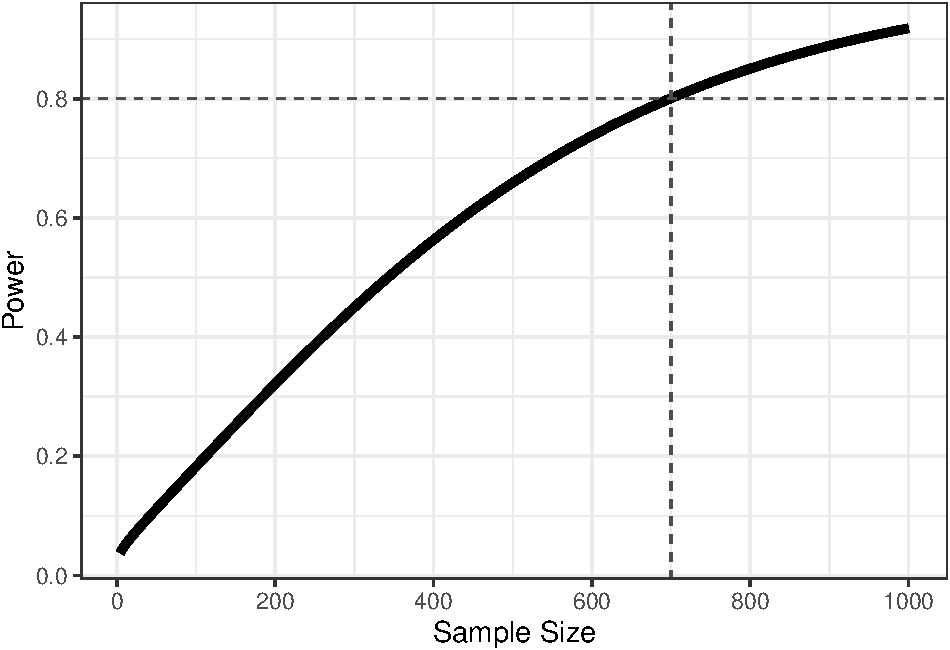
\includegraphics{power_simulation_files/figure-latex/power-figure-1.pdf}
\caption{\label{fig:power-figure}Power estimates for an effect size of 0.15 in the two-sample design.}
\end{figure}

\hypertarget{power-curves}{%
\subsection{Power Curves}\label{power-curves}}

It is common for the effect size of interest to not be completely certain a priori. In these cases, descriptive power analyses are often conducted that vary the effect size as well as the sample size to explore the power estimates for different effect sizes across a variety of sample sizes.

A similar structure can be done to add the power curves for different effect sizes; the primary differences being the addition of different effect sizes in addition to the different sample size conditions. These conditions are created using the \texttt{expand.grid} function which creates a row for each unique value of the variables specified. These conditions are then passed to the \texttt{power.t.test} function one at a time to create power estimates for each of the data conditions.

\begin{Shaded}
\begin{Highlighting}[]
\NormalTok{effect_sizes <-}\StringTok{ }\KeywordTok{c}\NormalTok{(.}\DecValTok{10}\NormalTok{, }\FloatTok{.15}\NormalTok{, }\FloatTok{.25}\NormalTok{)}
\NormalTok{conditions <-}\StringTok{ }\KeywordTok{expand.grid}\NormalTok{(}\DataTypeTok{n =}\NormalTok{ n, }\DataTypeTok{effect_sizes =}\NormalTok{ effect_sizes)}

\NormalTok{power_curve <-}\StringTok{ }\KeywordTok{sapply}\NormalTok{(}\KeywordTok{seq_len}\NormalTok{(}\KeywordTok{nrow}\NormalTok{(conditions)), }\ControlFlowTok{function}\NormalTok{(i) }
  \KeywordTok{power.t.test}\NormalTok{(}\DataTypeTok{n =}\NormalTok{ conditions[i, }\StringTok{'n'}\NormalTok{], }
               \DataTypeTok{delta =}\NormalTok{ conditions[i, }\StringTok{'effect_sizes'}\NormalTok{], }
               \DataTypeTok{sd =} \DecValTok{1}\NormalTok{, }\DataTypeTok{type =} \StringTok{'two.sample'}\NormalTok{)}\OperatorTok{$}\NormalTok{power)}
\end{Highlighting}
\end{Shaded}

A similar process is used to create a data frame with the conditions and power estimates to be visualized. Figure \ref{fig:vis-power-curve} shows the three power curves based on the three effects sizes of 0.10, 0.15, and 0.25. You'll notice that for the effect size of 0.10, estimated power never reaches the desired threshold of 0.80 indicating that larger sample sizes for each group would be needed. In addition, power estimates for an effect size of 0.25 reaches the threshold of 0.80 with around 250 individuals in each group. Having sample sizes much larger than that results in much smaller changes to the estimated power.

\begin{Shaded}
\begin{Highlighting}[]
\NormalTok{power_curve_df <-}\StringTok{ }\KeywordTok{bind_cols}\NormalTok{(}
\NormalTok{  conditions, }
  \DataTypeTok{power =}\NormalTok{ power_curve}
\NormalTok{)}

\KeywordTok{ggplot}\NormalTok{(power_curve_df, }\KeywordTok{aes}\NormalTok{(}\DataTypeTok{x =}\NormalTok{ n, }\DataTypeTok{y =}\NormalTok{ power)) }\OperatorTok{+}\StringTok{ }
\StringTok{  }\KeywordTok{geom_line}\NormalTok{(}\KeywordTok{aes}\NormalTok{(}\DataTypeTok{color =} \KeywordTok{factor}\NormalTok{(effect_sizes)), }\DataTypeTok{size =} \DecValTok{2}\NormalTok{) }\OperatorTok{+}\StringTok{ }
\StringTok{  }\KeywordTok{geom_hline}\NormalTok{(}\DataTypeTok{yintercept =} \FloatTok{0.8}\NormalTok{, }\DataTypeTok{linetype =} \DecValTok{2}\NormalTok{, }\DataTypeTok{color =} \StringTok{'gray30'}\NormalTok{) }\OperatorTok{+}\StringTok{ }
\StringTok{  }\KeywordTok{scale_x_continuous}\NormalTok{(}\StringTok{"Sample Size"}\NormalTok{, }\DataTypeTok{breaks =} \KeywordTok{seq}\NormalTok{(}\DecValTok{0}\NormalTok{, }\DecValTok{1000}\NormalTok{, }\DecValTok{200}\NormalTok{)) }\OperatorTok{+}\StringTok{ }
\StringTok{  }\KeywordTok{scale_y_continuous}\NormalTok{(}\StringTok{"Power"}\NormalTok{, }\DataTypeTok{breaks =} \KeywordTok{seq}\NormalTok{(}\DecValTok{0}\NormalTok{, }\DecValTok{1}\NormalTok{, }\FloatTok{.2}\NormalTok{)) }\OperatorTok{+}
\StringTok{  }\KeywordTok{scale_color_grey}\NormalTok{(}\StringTok{"Effect Size"}\NormalTok{) }\OperatorTok{+}
\StringTok{  }\KeywordTok{theme_bw}\NormalTok{(}\DataTypeTok{base_size =} \DecValTok{14}\NormalTok{)}
\end{Highlighting}
\end{Shaded}

\begin{figure}
\centering
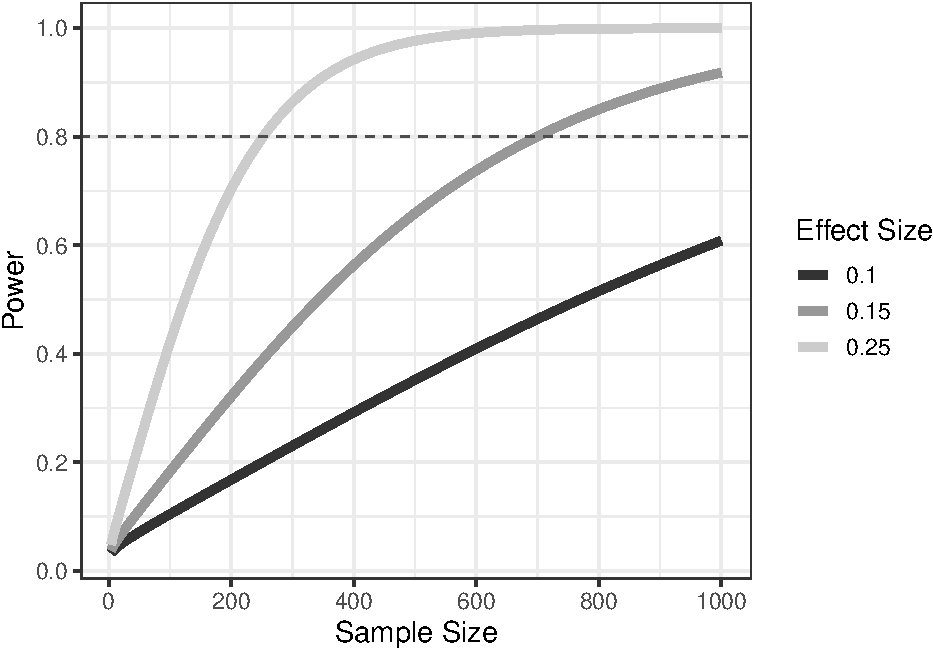
\includegraphics{power_simulation_files/figure-latex/vis-power-curve-1.pdf}
\caption{\label{fig:vis-power-curve}Three power curves representing power estimates across three different effect sizes and various sample sizes.}
\end{figure}

\hypertarget{two-sample-data-simulation-with-simglm}{%
\section{\texorpdfstring{Two sample Data simulation with \texttt{simglm}}{Two sample Data simulation with simglm}}\label{two-sample-data-simulation-with-simglm}}

The same two sample power analysis can be conducted by simulation with the \texttt{simglm} R package (LeBeau, 2019). This package simulates data based on general(-ized) linear (mixed) models and can replicate the simulation procedure to perform a power analysis. In order to use the \texttt{simglm} package, the two-sample t-test described above needs to be reformulated into an equivalent form using the general linear model or more specifically a linear regression model.

The linear regression model would look like the following:
\begin{equation} 
Y_{i} = \beta_{0} + \beta_{1} group_{i} + \epsilon_{i} 
\label{eq:twosamp}
\end{equation}

\noindent where \(Y_{i}\) is the outcome of interest (i.e.~reading or depression scores reference above) for individual \(i\), \(group_{i}\) is a fixed indicator variable that would have a score of 1 if an individual belonged to group 1 otherwise would have a score of 0, and \(\epsilon_{i}\) would represent random sampling error. With the linear regression model set up this way, \(\beta_{0}\) would represent the intercept and would be interpreted as the mean of the group coded as 0 in the \(group_{i}\) variable. The second coefficient, \(\beta_{1}\), would be the variable of interest and represent the mean difference between the two groups. The mean of the second group could be found by taking \(\beta_{0} + \beta_{1}\). The primary benefit of approaching the two-sample t-test in this fashion is the model specification flexiblity, in particular if statistical controls or interactions would want to be explored.

The following code is an example of simulating data using the \texttt{simglm} package. The code consists of two parts, the first part specifies the parameters for the simulation in a named list, named \texttt{simulation\_arguments} below. For the two-sample linear regression model shown above the following named elements need to be included, the model formula (which mimics the linear regression formula depicted above without the error), the fixed component representing the group variable (depicted as sex below), the sample size (i.e.~how many individuals), the size of random error variance, and the regression weights. The regression weights (named \texttt{reg\_weights} below) represent the values for \(\beta_{0}\) and \(\beta_{1}\) discussed above. Exploring the code below, this would mean that the mean for group 1 would be assumed to be 0 and the mean difference between the two groups is 0.15 (equivalently here the mean of group 2 would be \(0 + 0.15 = 0.15\)). Since the error variance is specified to equal 1, the data generated mimics a standardized example and the interpretation of the second regression weight (i.e.~\(\beta_{1} = 0.15\)) would be similar to the effect size cohen's d.~

Finally, the fixed argument in some cases will be the most difficult argument to specify and often requires the most code. In this example, only the sex variable needs to be defined how this should be simulated. The code for the fixed portion identifies that this variable should be a factor variable, using the \texttt{var\_type} argument and the levels of the sex variable (i.e.~male and female) are specified. This ensures that the data labels are created directly rather than just numeric values and can be helpful to ensure the creation of the two groups. Internally during the simulation process this variable with character labels would be turned into a dichotomous indicator variable that is defined above in Equation \eqref{eq:twosamp}.

\begin{Shaded}
\begin{Highlighting}[]
\NormalTok{simulation_arguments <-}\StringTok{ }\KeywordTok{list}\NormalTok{(}
  \DataTypeTok{formula =}\NormalTok{ y }\OperatorTok{~}\StringTok{ }\DecValTok{1} \OperatorTok{+}\StringTok{ }\NormalTok{sex,}
  \DataTypeTok{fixed =} \KeywordTok{list}\NormalTok{(}\DataTypeTok{sex =} \KeywordTok{list}\NormalTok{(}\DataTypeTok{var_type =} \StringTok{'factor'}\NormalTok{, }
                            \DataTypeTok{levels =} \KeywordTok{c}\NormalTok{(}\StringTok{'male'}\NormalTok{, }\StringTok{'female'}\NormalTok{))),}
  \DataTypeTok{sample_size =} \DecValTok{20}\NormalTok{,}
  \DataTypeTok{error =} \KeywordTok{list}\NormalTok{(}\DataTypeTok{variance =} \DecValTok{1}\NormalTok{),}
  \DataTypeTok{reg_weights =} \KeywordTok{c}\NormalTok{(}\DecValTok{0}\NormalTok{, }\FloatTok{.15}\NormalTok{)}
\NormalTok{)}
\end{Highlighting}
\end{Shaded}

A series of commands are used for the generation of the simulated data, \texttt{simulate\_fixed}, \texttt{simulate\_error}, and \texttt{generate\_response}. In general these function take the simulation arguments defined in the previous code chunk as the primary argument and the \texttt{\%\textgreater{}\%} pipe operator is used to chain the commands together which passes the result from the previous step to the first function argument which for the simglm package is always the data. The \texttt{simulate\_fixed} function generates the fixed portion of the model which for the model shown in Equation \eqref{eq:twosamp} representing the intercept and sex variables respectively. The \texttt{simulate\_error} function generates the random sampling error and \texttt{generate\_response} takes the results from the first two functions to generate the outcome.

\begin{Shaded}
\begin{Highlighting}[]
\KeywordTok{simulate_fixed}\NormalTok{(}\DataTypeTok{data =} \OtherTok{NULL}\NormalTok{, simulation_arguments) }\OperatorTok
\StringTok{  }\KeywordTok{simulate_error}\NormalTok{(simulation_arguments) }\OperatorTok
\StringTok{  }\KeywordTok{generate_response}\NormalTok{(simulation_arguments)}
\end{Highlighting}
\end{Shaded}

Table \ref{tab:simulate-data-out} shows the first six rows of the simulated data. The output shows the values for the sex variable which would represent the variable of interest and the outcome variable here is represented as the last column labeled y. The random error values are also given in the error column. It is useful to explore the simulated data prior to going to simulation to ensure that was in simulated is what was specified. In addition, the output in Table \ref{tab:simulat-data-out} shows the the mean difference of 0.15 would indicate that males are 0.15 standard units higher than females. If the opposite would want to be created, the parameter in the \texttt{reg\_weights} argument could be made negative (i.e.~-0.15) which would indicate males have a smaller mean.

\begin{table}[t]

\caption{\label{tab:simulate-data-out}The output from the simulated data generated with simglm}
\centering
\begin{tabular}{rrlrrrrr}
\toprule
X.Intercept. & sex & sex1 & level1\_id & error & fixed\_outcome & random\_effects & y\\
\midrule
1 & 1 & male & 1 & 2.29 & 0.15 & 0 & 2.44\\
1 & 1 & male & 2 & -1.39 & 0.15 & 0 & -1.24\\
1 & 0 & female & 3 & -0.28 & 0.00 & 0 & -0.28\\
1 & 0 & female & 4 & -0.13 & 0.00 & 0 & -0.13\\
1 & 0 & female & 5 & 0.64 & 0.00 & 0 & 0.64\\
\addlinespace
1 & 0 & female & 6 & -0.28 & 0.00 & 0 & -0.28\\
\bottomrule
\end{tabular}
\end{table}

\hypertarget{using-simglm-to-generate-power}{%
\subsection{\texorpdfstring{Using \texttt{simglm} to generate power}{Using simglm to generate power}}\label{using-simglm-to-generate-power}}

Very few adjustments are need to generate power using the \texttt{simglm} package once the simulation code is added. The number of replications need to be specified, a specification of what kind of model should be fitted, and whether to extract the model coefficients. The number of replications indicate how many times the data will be simulated and subsequently how many times model estimates will be obtained. In general, larger is better and will increase precision in the power estimates that are obtained. The number of replications can be thought of as similar to sample size in primary studies. In the example below, the number of replications is set to 1000 which is a minimum value that I would recommend and was used here as a trade-off between time to run the power analysis and precision of the power estimates. The more replications that are run, the longer the power analysis will take to run.

The model to be fitted is specified with the names \texttt{model\_fit} argument. Only the \texttt{model\_function} needs to be specified within the \texttt{model\_fit} list to indicate which R model function should be used. The additional argument of model formula is also shown below as this gives the user additional flexibility and would allow the user to explore the impact of model misspecification (i.e.~not including a model variable that is present in the population). If the model formula is omitted from the \texttt{model\_fit} argument, the same model formula as the simulated model is specified. Finally, the \texttt{extract\_coefficients} is commonly specified as TRUE to indicate that the estimated coefficients from the fitting of models from \texttt{model\_fit} will be returned. If the \texttt{extract\_coefficients} argument is missing from the simulation arguments, then the fitted model object is returned which would need to be processed to extract relavent information.

\begin{Shaded}
\begin{Highlighting}[]
\KeywordTok{plan}\NormalTok{(multiprocess)}

\NormalTok{simulation_arguments <-}\StringTok{ }\KeywordTok{list}\NormalTok{(}
  \DataTypeTok{formula =}\NormalTok{ y }\OperatorTok{~}\StringTok{ }\DecValTok{1} \OperatorTok{+}\StringTok{ }\NormalTok{sex,}
  \DataTypeTok{fixed =} \KeywordTok{list}\NormalTok{(}\DataTypeTok{sex =} \KeywordTok{list}\NormalTok{(}\DataTypeTok{var_type =} \StringTok{'factor'}\NormalTok{, }
                            \DataTypeTok{levels =} \KeywordTok{c}\NormalTok{(}\StringTok{'male'}\NormalTok{, }\StringTok{'female'}\NormalTok{))),}
  \DataTypeTok{sample_size =} \DecValTok{20}\NormalTok{,}
  \DataTypeTok{error =} \KeywordTok{list}\NormalTok{(}\DataTypeTok{variance =} \DecValTok{1}\NormalTok{),}
  \DataTypeTok{reg_weights =} \KeywordTok{c}\NormalTok{(}\DecValTok{0}\NormalTok{, }\FloatTok{.15}\NormalTok{),}
  \DataTypeTok{replications =} \DecValTok{1000}\NormalTok{,}
  \DataTypeTok{model_fit =} \KeywordTok{list}\NormalTok{(}\DataTypeTok{formula =}\NormalTok{ y }\OperatorTok{~}\StringTok{ }\DecValTok{1} \OperatorTok{+}\StringTok{ }\NormalTok{sex, }
                   \DataTypeTok{model_function =} \StringTok{'lm'}\NormalTok{),}
  \DataTypeTok{extract_coefficients =} \OtherTok{TRUE}
\NormalTok{)}

\NormalTok{replicate_sim <-}\StringTok{ }\KeywordTok{replicate_simulation}\NormalTok{(simulation_arguments)}
\end{Highlighting}
\end{Shaded}

Finally, one last function is needed to compute power and other useful summary statistics based on the analysis. The \texttt{compute\_statistics} function is used to compute these summary statistics from the replicated simulation results. The primary arguments for this function include the simulation arguments and which statistics to be returned. In the example below, power and precision are set to TRUE to return those statistics and type I error statistics are omitted as power is of most interest here. For simulation studies to explore methodological impacts of assumption violations, type I error may be of interest to users.

\begin{Shaded}
\begin{Highlighting}[]
\NormalTok{replicate_sim }\OperatorTok
\StringTok{  }\KeywordTok{compute_statistics}\NormalTok{(simulation_arguments, }\DataTypeTok{power =} \OtherTok{TRUE}\NormalTok{,}
                     \DataTypeTok{type_1_error =} \OtherTok{FALSE}\NormalTok{, }\DataTypeTok{precision =} \OtherTok{TRUE}\NormalTok{)}
\end{Highlighting}
\end{Shaded}

Table \ref{tab:compute-stat-tab} shows the output from the power analysis with simglm. The output shows the information for power and precision. In the output, if power estimates are of most concern, the columns \enquote{Avg Est} and \enquote{Power} are most relavent which provide estimates for the average estimates and the number of binary hypotheses correctly rejected across all replications. The additional information is more for reference, but contain information on the average test statistic, parameter estimate standard deviation, average standard error, precision (estimated standard deviation / average standard error), and number of replications. In the example shown above with only a sample size of 20 individuals, the estimated power was 0.08 meaning that the null hypothesis would only be correctly rejected 8\% of the time.

\begin{table}[t]

\caption{\label{tab:compute-stat-tab}Statistical power and precision output obtained from the simglm package.}
\centering
\begin{tabular}{lrrrrrrr}
\toprule
Term & Avg Est & Power & Avg TS & Est SD & Avg SE & Precision & Repl\\
\midrule
(Intercept) & 0.01 & 0.08 & 0.04 & 0.33 & 0.32 & 1.02 & 1000\\
sex & 0.13 & 0.08 & 0.30 & 0.46 & 0.46 & 1.01 & 1000\\
\bottomrule
\end{tabular}
\end{table}

\hypertarget{varying-arguments-with-simglm}{%
\subsection{\texorpdfstring{Varying arguments with \texttt{simglm}}{Varying arguments with simglm}}\label{varying-arguments-with-simglm}}

The example with \texttt{simglm} above only considered power for a single sample size, but a power-curve was shown above that reflected various sample sizes and various effect sizes simultaneously. This can be achieved in a single analysis by using the \texttt{vary\_arguments} argument to the simulation arguments. As shown in the code below, the \texttt{sample\_size} argument is removed from the main simulation arguments and it is instead specified within the \texttt{vary\_arguments} argument. The sample size is generated to indicate that the sample size should be evaluated for the sequence starting at 20, ending at 2000, and incrementing by 20. When specifying arguments to vary, the default behavior is to do a factorial design meaning that all combinations are considered and replicated as part of the power analysis. More specifically for this example, this would mean that sample sizes of 20, 40, 60, up to 2000 will be run and replicated 1000 times.

Finally, an optional argument named, \texttt{power}, is shown that provides further user customization to how power is calculated. For example, the power arguments defined below indicate that a standard normal critical value with an alpha value of 0.05 and the default behavior is to assume a two-tailed hypothesis test. Therefore, the test statistics estimated from the model fitting will be compared to a critical value of \(\pm 1.96\). This was used here for its simplicity, but it is acknowledged that this may result in conservative estimates of power for smaller sample sizes. In these cases a t-distribution may be more appropriate.

\begin{Shaded}
\begin{Highlighting}[]
\NormalTok{simulation_arguments <-}\StringTok{ }\KeywordTok{list}\NormalTok{(}
  \DataTypeTok{formula =}\NormalTok{ y }\OperatorTok{~}\StringTok{ }\DecValTok{1} \OperatorTok{+}\StringTok{ }\NormalTok{sex, }
  \DataTypeTok{fixed =} \KeywordTok{list}\NormalTok{(}\DataTypeTok{sex =} \KeywordTok{list}\NormalTok{(}\DataTypeTok{var_type =} \StringTok{'factor'}\NormalTok{, }
                            \DataTypeTok{levels =} \KeywordTok{c}\NormalTok{(}\StringTok{'male'}\NormalTok{, }\StringTok{'female'}\NormalTok{))),}
  \DataTypeTok{error =} \KeywordTok{list}\NormalTok{(}\DataTypeTok{variance =} \DecValTok{1}\NormalTok{),}
  \DataTypeTok{reg_weights =} \KeywordTok{c}\NormalTok{(}\DecValTok{0}\NormalTok{, }\FloatTok{.15}\NormalTok{),}
  \DataTypeTok{replications =} \DecValTok{1000}\NormalTok{,}
  \DataTypeTok{model_fit =} \KeywordTok{list}\NormalTok{(}\DataTypeTok{formula =}\NormalTok{ y }\OperatorTok{~}\StringTok{ }\DecValTok{1} \OperatorTok{+}\StringTok{ }\NormalTok{sex,}
                   \DataTypeTok{model_function =} \StringTok{'lm'}\NormalTok{),}
  \DataTypeTok{power =} \KeywordTok{list}\NormalTok{(}
    \DataTypeTok{dist =} \StringTok{'qnorm'}\NormalTok{,}
    \DataTypeTok{alpha =} \FloatTok{.05}
\NormalTok{  ),}
  \DataTypeTok{extract_coefficients =} \OtherTok{TRUE}\NormalTok{,}
  \DataTypeTok{vary_arguments =} \KeywordTok{list}\NormalTok{(}
    \DataTypeTok{sample_size =} \KeywordTok{seq}\NormalTok{(}\DecValTok{20}\NormalTok{, }\DecValTok{2000}\NormalTok{, }\DecValTok{20}\NormalTok{) }
\NormalTok{  )}
\NormalTok{)}

\NormalTok{model_results <-}\StringTok{ }\KeywordTok{replicate_simulation}\NormalTok{(simulation_arguments) }
\end{Highlighting}
\end{Shaded}

The \texttt{compute\_statistics} function is again used to generate summary statistics. Internally, the arguments that are varied are used as grouping variables when computing these summary statistics, therefore power values will be computed for all unique values for arguments that were varied. In addition, some post-processing is done to turn the sample size values from a factor variable to numeric for easier use later on and only the power values for the sex variable are returned as this is the power effect of interest.

\begin{Shaded}
\begin{Highlighting}[]
\NormalTok{power_results <-}\StringTok{ }\NormalTok{model_results }\OperatorTok
\StringTok{  }\KeywordTok{compute_statistics}\NormalTok{(simulation_arguments, }\DataTypeTok{power =} \OtherTok{TRUE}\NormalTok{,}
                     \DataTypeTok{type_1_error =} \OtherTok{FALSE}\NormalTok{, }\DataTypeTok{precision =} \OtherTok{TRUE}\NormalTok{)}

\NormalTok{power_results <-}\StringTok{ }\NormalTok{power_results }\OperatorTok
\StringTok{  }\KeywordTok{ungroup}\NormalTok{() }\OperatorTok
\StringTok{  }\KeywordTok{mutate}\NormalTok{(}\DataTypeTok{sample_size =} \KeywordTok{as.numeric}\NormalTok{(}\KeywordTok{as.character}\NormalTok{(sample_size))) }\OperatorTok
\StringTok{  }\KeywordTok{arrange}\NormalTok{(sample_size) }\OperatorTok
\StringTok{  }\KeywordTok{filter}\NormalTok{(term }\OperatorTok{==}\StringTok{ 'sex'}\NormalTok{)}
\end{Highlighting}
\end{Shaded}

The tabular results could be explored by viewing the \texttt{power\_results} object directly, however this would be more difficult to interpret quickly. Therefore, the result can then be explored visually to generate a power curve across the sample sizes for this single effect size. The results mimic was would found in Figure \ref{fig:power-figure} where sample sizes for each group was approximately 700.

\begin{Shaded}
\begin{Highlighting}[]
\KeywordTok{ggplot}\NormalTok{(power_results, }\KeywordTok{aes}\NormalTok{(}\DataTypeTok{x =}\NormalTok{ sample_size, }\DataTypeTok{y =}\NormalTok{ power)) }\OperatorTok{+}\StringTok{ }
\StringTok{  }\KeywordTok{geom_point}\NormalTok{(}\DataTypeTok{size =} \FloatTok{1.5}\NormalTok{, }\DataTypeTok{color =} \StringTok{'gray40'}\NormalTok{) }\OperatorTok{+}\StringTok{ }
\StringTok{  }\KeywordTok{geom_hline}\NormalTok{(}\DataTypeTok{yintercept =} \FloatTok{0.8}\NormalTok{, }\DataTypeTok{linetype =} \DecValTok{2}\NormalTok{, }\DataTypeTok{color =} \StringTok{'gray30'}\NormalTok{) }\OperatorTok{+}\StringTok{ }
\StringTok{  }\KeywordTok{geom_smooth}\NormalTok{(}\DataTypeTok{linetype =} \DecValTok{1}\NormalTok{, }\DataTypeTok{size =} \DecValTok{1}\NormalTok{, }\DataTypeTok{se =} \OtherTok{FALSE}\NormalTok{) }\OperatorTok{+}
\StringTok{  }\KeywordTok{geom_vline}\NormalTok{(}\DataTypeTok{xintercept =} \KeywordTok{min}\NormalTok{(}\KeywordTok{filter}\NormalTok{(power_results, power }\OperatorTok{>=}\StringTok{ }\FloatTok{0.8}\NormalTok{)}\OperatorTok{$}\NormalTok{power), }\DataTypeTok{linetype =} \DecValTok{2}\NormalTok{, }\DataTypeTok{color =} \StringTok{'gray30'}\NormalTok{) }\OperatorTok{+}
\StringTok{  }\KeywordTok{scale_x_continuous}\NormalTok{(}\StringTok{"Sample Size"}\NormalTok{, }\DataTypeTok{breaks =} \KeywordTok{seq}\NormalTok{(}\DecValTok{0}\NormalTok{, }\DecValTok{2000}\NormalTok{, }\DecValTok{200}\NormalTok{)) }\OperatorTok{+}\StringTok{ }
\StringTok{  }\KeywordTok{scale_y_continuous}\NormalTok{(}\StringTok{"Power"}\NormalTok{, }\DataTypeTok{breaks =} \KeywordTok{seq}\NormalTok{(}\DecValTok{0}\NormalTok{, }\DecValTok{1}\NormalTok{, }\FloatTok{.2}\NormalTok{)) }\OperatorTok{+}
\StringTok{  }\KeywordTok{theme_bw}\NormalTok{(}\DataTypeTok{base_size =} \DecValTok{14}\NormalTok{)}
\end{Highlighting}
\end{Shaded}

\begin{figure}
\centering
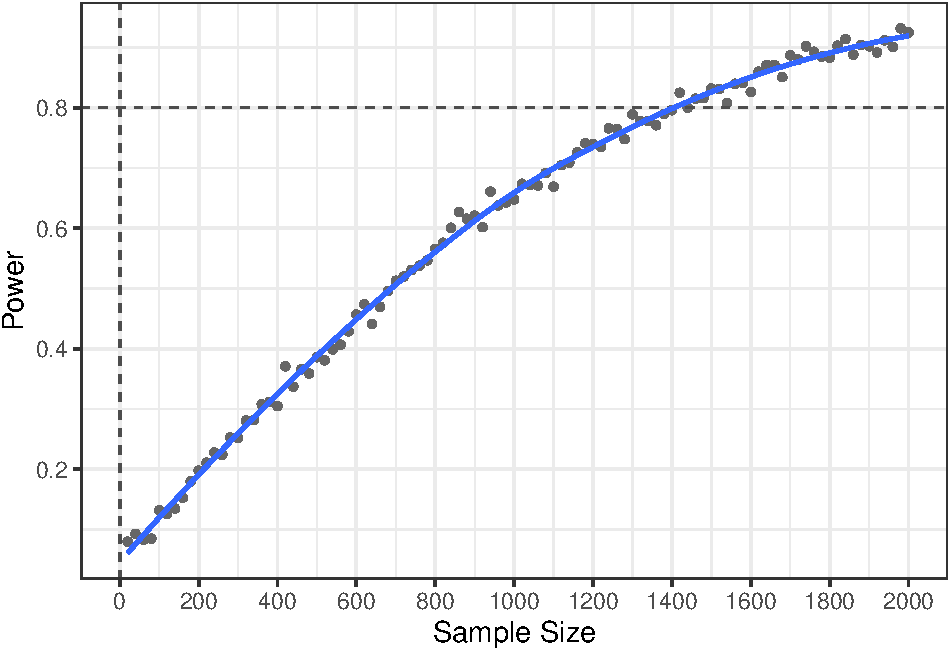
\includegraphics{power_simulation_files/figure-latex/simglm-power-curve-1.pdf}
\caption{\label{fig:simglm-power-curve}A single power curve for varying sample size conditions with a single effect size using simglm.}
\end{figure}

\hypertarget{visualizing-estimates-and-p-values}{%
\subsection{Visualizing estimates and p-values}\label{visualizing-estimates-and-p-values}}

Exploring the estimates and the p-values can be informative over and above the power graphics shown above. The model results are stored in the object, \texttt{model\_results} shown above as a list for each replicated condition. This means that for each sample size, there are 1000 estimates for the sex effect and the associated p-values based on these.

The \texttt{model\_results} object is a list across sample size conditions, therefore this is first combined into a dataframe and then plotted with ggplot2. The resulting figure shows the increased precision as sample size increases. More specifically, the standard error is decreasing, but on average the parameter estimate is centered around 0.15.

\begin{Shaded}
\begin{Highlighting}[]
\NormalTok{model_results_df <-}\StringTok{ }\KeywordTok{bind_rows}\NormalTok{(model_results) }\OperatorTok
\StringTok{  }\KeywordTok{filter}\NormalTok{(term }\OperatorTok{==}\StringTok{ 'sex'}\NormalTok{) }\OperatorTok
\StringTok{  }\KeywordTok{mutate}\NormalTok{(}\DataTypeTok{sample_size =} \KeywordTok{as.numeric}\NormalTok{(}\KeywordTok{as.character}\NormalTok{(sample_size)))}

\KeywordTok{ggplot}\NormalTok{(model_results_df, }\KeywordTok{aes}\NormalTok{(}\DataTypeTok{x =}\NormalTok{ sample_size, }\DataTypeTok{y =}\NormalTok{ estimate)) }\OperatorTok{+}\StringTok{ }
\StringTok{  }\KeywordTok{geom_boxplot}\NormalTok{(}\KeywordTok{aes}\NormalTok{(}\DataTypeTok{group =}\NormalTok{ sample_size), }\DataTypeTok{outlier.alpha =} \FloatTok{0.01}\NormalTok{) }\OperatorTok{+}
\StringTok{  }\KeywordTok{scale_x_continuous}\NormalTok{(}\StringTok{"Sample Size"}\NormalTok{, }\DataTypeTok{breaks =} \KeywordTok{seq}\NormalTok{(}\DecValTok{0}\NormalTok{, }\DecValTok{2000}\NormalTok{, }\DecValTok{200}\NormalTok{)) }\OperatorTok{+}
\StringTok{  }\KeywordTok{theme_bw}\NormalTok{(}\DataTypeTok{base_size =} \DecValTok{14}\NormalTok{) }\OperatorTok{+}
\StringTok{  }\KeywordTok{geom_hline}\NormalTok{(}\DataTypeTok{yintercept =} \FloatTok{.15}\NormalTok{, }\DataTypeTok{linetype =} \DecValTok{2}\NormalTok{, }\DataTypeTok{size =} \DecValTok{2}\NormalTok{, }\DataTypeTok{color =} \StringTok{'gray20'}\NormalTok{) }\OperatorTok{+}
\StringTok{  }\KeywordTok{coord_flip}\NormalTok{()}
\end{Highlighting}
\end{Shaded}

\begin{figure}
\centering
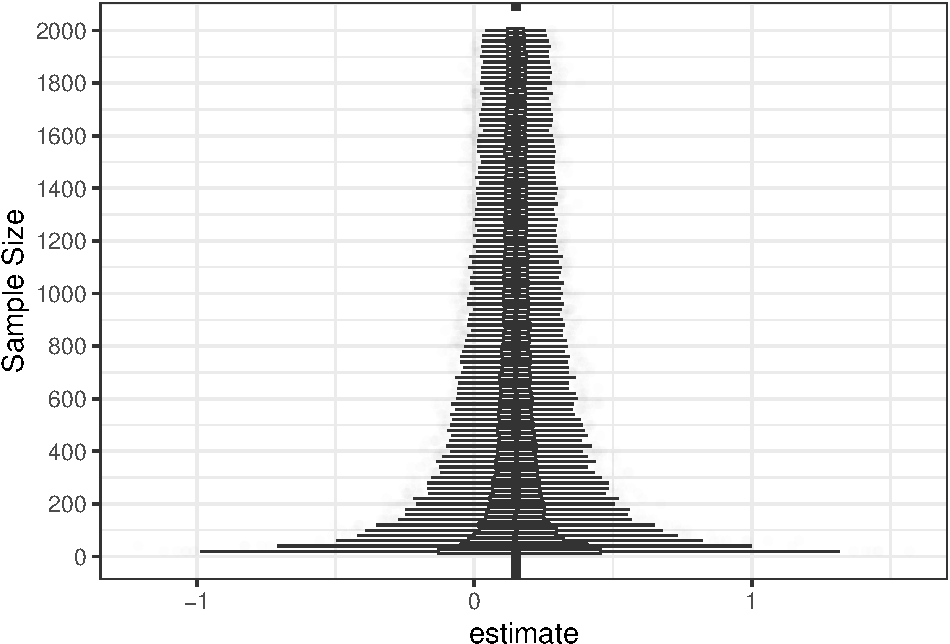
\includegraphics{power_simulation_files/figure-latex/estimate-figure-1.pdf}
\caption{\label{fig:estimate-figure}Distribution of parameter estimates for the sex effect by sample size.}
\end{figure}

A similar figure can be created showing the distribution of p-values, which gives a similar picture. There is much more variation when the sample sizes are small compared to larger sample sizes which reflects the smaller standard errors.

\begin{Shaded}
\begin{Highlighting}[]
\KeywordTok{ggplot}\NormalTok{(model_results_df, }\KeywordTok{aes}\NormalTok{(}\DataTypeTok{x =}\NormalTok{ sample_size, }\DataTypeTok{y =}\NormalTok{ p.value)) }\OperatorTok{+}\StringTok{ }
\StringTok{  }\KeywordTok{geom_boxplot}\NormalTok{(}\KeywordTok{aes}\NormalTok{(}\DataTypeTok{group =}\NormalTok{ sample_size), }\DataTypeTok{outlier.alpha =} \FloatTok{0.01}\NormalTok{) }\OperatorTok{+}
\StringTok{  }\KeywordTok{scale_x_continuous}\NormalTok{(}\StringTok{"Sample Size"}\NormalTok{, }\DataTypeTok{breaks =} \KeywordTok{seq}\NormalTok{(}\DecValTok{0}\NormalTok{, }\DecValTok{2000}\NormalTok{, }\DecValTok{200}\NormalTok{)) }\OperatorTok{+}
\StringTok{  }\KeywordTok{ylab}\NormalTok{(}\StringTok{"p-value"}\NormalTok{) }\OperatorTok{+}
\StringTok{  }\KeywordTok{theme_bw}\NormalTok{(}\DataTypeTok{base_size =} \DecValTok{14}\NormalTok{) }\OperatorTok{+}
\StringTok{  }\KeywordTok{geom_hline}\NormalTok{(}\DataTypeTok{yintercept =} \FloatTok{.05}\NormalTok{, }\DataTypeTok{linetype =} \DecValTok{2}\NormalTok{, }\DataTypeTok{size =} \DecValTok{2}\NormalTok{, }\DataTypeTok{color =} \StringTok{'gray20'}\NormalTok{) }\OperatorTok{+}
\StringTok{  }\KeywordTok{coord_flip}\NormalTok{()}
\end{Highlighting}
\end{Shaded}

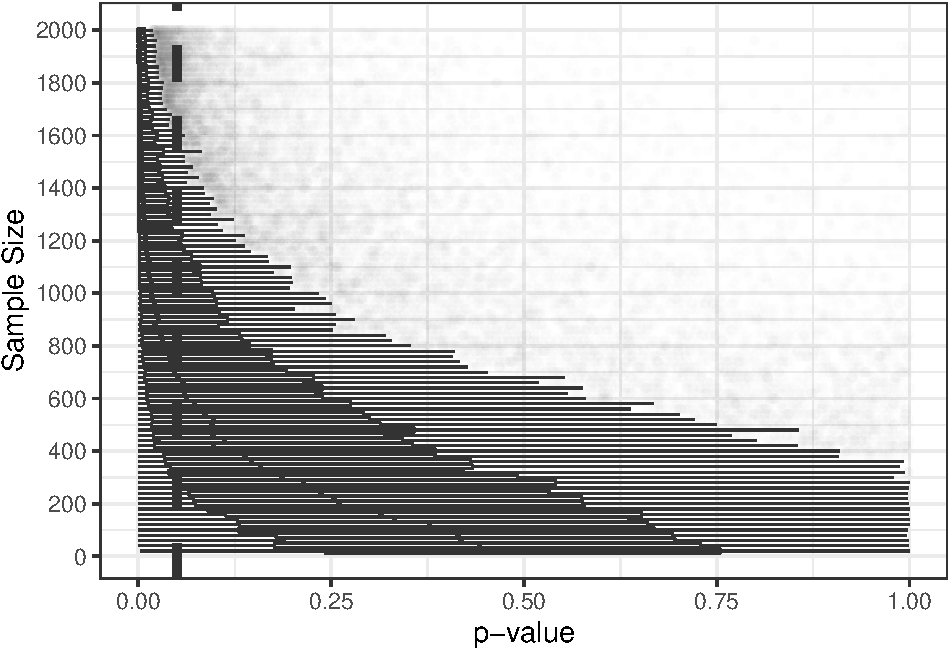
\includegraphics{power_simulation_files/figure-latex/p-value-figure-1.pdf}

\hypertarget{add-heterogeneity}{%
\subsection{Add Heterogeneity}\label{add-heterogeneity}}

Heterogeneity is a common phenomenon that can impact power and can occur when there are population variance differences across the two groups. In the above example, this would mean that there would be variance differences across males and females, perhaps males are more variable in the outcome. The \texttt{power.t.test} function from before does not assume heterogeneity, however this is possible to incorporate when doing power from a simulation framework. Adding these conditions can help to mimic real world conditions and also maybe provide a better estimate of power.

To simulate heterogeneity an additional argument to the simulation arguments is added called \texttt{heterogeneity}. This argument species the group to which the heterogeneity is applied, in this case the group/sex variable and the specific variances for the values of that variable. In this example, there are only two groups therefore only two variances need to be supplied. The variance for the second group is set to be about 8 times that of the first group, a ratio that exceeds a common heuristic of 3 times variance ratio indicating a violation of the statistical assumption homogeneity of variance.

\begin{Shaded}
\begin{Highlighting}[]
\NormalTok{simulation_arguments <-}\StringTok{ }\KeywordTok{list}\NormalTok{(}
  \DataTypeTok{formula =}\NormalTok{ y }\OperatorTok{~}\StringTok{ }\DecValTok{1} \OperatorTok{+}\StringTok{ }\NormalTok{group,}
  \DataTypeTok{fixed =} \KeywordTok{list}\NormalTok{(}\DataTypeTok{group =} \KeywordTok{list}\NormalTok{(}\DataTypeTok{var_type =} \StringTok{'factor'}\NormalTok{, }
                            \DataTypeTok{levels =} \KeywordTok{c}\NormalTok{(}\StringTok{'male'}\NormalTok{, }\StringTok{'female'}\NormalTok{))),}
  \DataTypeTok{error =} \KeywordTok{list}\NormalTok{(}\DataTypeTok{variance =} \DecValTok{1}\NormalTok{),}
  \DataTypeTok{heterogeneity =} \KeywordTok{list}\NormalTok{(}\DataTypeTok{variable =} \StringTok{'group'}\NormalTok{,}
                       \DataTypeTok{variance =} \KeywordTok{c}\NormalTok{(}\DecValTok{1}\NormalTok{, }\DecValTok{8}\NormalTok{)),}
  \DataTypeTok{reg_weights =} \KeywordTok{c}\NormalTok{(}\DecValTok{0}\NormalTok{, }\FloatTok{.15}\NormalTok{),}
  \DataTypeTok{replications =} \DecValTok{1000}\NormalTok{,}
  \DataTypeTok{model_fit =} \KeywordTok{list}\NormalTok{(}\DataTypeTok{formula =}\NormalTok{ y }\OperatorTok{~}\StringTok{ }\DecValTok{1} \OperatorTok{+}\StringTok{ }\NormalTok{group, }
                   \DataTypeTok{model_function =} \StringTok{'lm'}\NormalTok{),}
  \DataTypeTok{power =} \KeywordTok{list}\NormalTok{(}
    \DataTypeTok{dist =} \StringTok{'qnorm'}\NormalTok{,}
    \DataTypeTok{alpha =} \FloatTok{.05}
\NormalTok{  ),}
  \DataTypeTok{extract_coefficients =} \OtherTok{TRUE}\NormalTok{,}
  \DataTypeTok{vary_arguments =} \KeywordTok{list}\NormalTok{(}
    \DataTypeTok{sample_size =} \KeywordTok{seq}\NormalTok{(}\DecValTok{20}\NormalTok{, }\DecValTok{2000}\NormalTok{, }\DecValTok{20}\NormalTok{) }
\NormalTok{  )}
\NormalTok{)}

\NormalTok{model_results_h <-}\StringTok{ }\KeywordTok{replicate_simulation}\NormalTok{(simulation_arguments)}
\end{Highlighting}
\end{Shaded}

These results are then processed similarly to above and combined with the power results that assumed a constant variance across the two groups. Figure \ref{fig:simglm-power-curve-h} shows the power estimates contrasting results with and without heterogeneity. The effect of heterogeneity is quite stark with significantly reduced power estimates when there is heterogeneity. Smaller variance ratios could be considered to explore smaller ratios and the results impact on power estimates.

\begin{Shaded}
\begin{Highlighting}[]
\NormalTok{power_results_h <-}\StringTok{ }\NormalTok{model_results_h }\OperatorTok
\StringTok{  }\KeywordTok{compute_statistics}\NormalTok{(simulation_arguments, }\DataTypeTok{power =} \OtherTok{TRUE}\NormalTok{,}
                     \DataTypeTok{type_1_error =} \OtherTok{FALSE}\NormalTok{, }\DataTypeTok{precision =} \OtherTok{TRUE}\NormalTok{) }\OperatorTok
\StringTok{  }\KeywordTok{ungroup}\NormalTok{() }\OperatorTok
\StringTok{  }\KeywordTok{mutate}\NormalTok{(}\DataTypeTok{sample_size =} \KeywordTok{as.numeric}\NormalTok{(}\KeywordTok{as.character}\NormalTok{(sample_size)),}
         \DataTypeTok{heterogeneity =} \OtherTok{TRUE}\NormalTok{) }\OperatorTok
\StringTok{  }\KeywordTok{arrange}\NormalTok{(sample_size) }\OperatorTok
\StringTok{  }\KeywordTok{filter}\NormalTok{(term }\OperatorTok{==}\StringTok{ 'group'}\NormalTok{)}

\NormalTok{power_results <-}\StringTok{ }\NormalTok{power_results }\OperatorTok
\StringTok{  }\KeywordTok{mutate}\NormalTok{(}\DataTypeTok{heterogeneity =} \OtherTok{FALSE}\NormalTok{)}

\NormalTok{power_results_combined <-}\StringTok{ }\KeywordTok{bind_rows}\NormalTok{(power_results, }
\NormalTok{                                    power_results_h)}
\end{Highlighting}
\end{Shaded}

\begin{Shaded}
\begin{Highlighting}[]
\KeywordTok{ggplot}\NormalTok{(power_results_combined, }\KeywordTok{aes}\NormalTok{(}\DataTypeTok{x =}\NormalTok{ sample_size, }\DataTypeTok{y =}\NormalTok{ power, }
                          \DataTypeTok{group =}\NormalTok{ heterogeneity)) }\OperatorTok{+}\StringTok{ }
\StringTok{  }\KeywordTok{geom_point}\NormalTok{(}\KeywordTok{aes}\NormalTok{(}\DataTypeTok{shape =}\NormalTok{ heterogeneity), }\DataTypeTok{size =} \FloatTok{1.5}\NormalTok{, }\DataTypeTok{color =} \StringTok{'gray40'}\NormalTok{) }\OperatorTok{+}\StringTok{ }
\StringTok{  }\KeywordTok{geom_hline}\NormalTok{(}\DataTypeTok{yintercept =} \FloatTok{0.8}\NormalTok{, }\DataTypeTok{linetype =} \DecValTok{2}\NormalTok{, }\DataTypeTok{color =} \StringTok{'gray30'}\NormalTok{) }\OperatorTok{+}\StringTok{ }
\StringTok{  }\KeywordTok{geom_smooth}\NormalTok{(}\KeywordTok{aes}\NormalTok{(}\DataTypeTok{linetype =}\NormalTok{ heterogeneity), }\DataTypeTok{size =} \DecValTok{1}\NormalTok{, }\DataTypeTok{se =} \OtherTok{FALSE}\NormalTok{) }\OperatorTok{+}
\StringTok{  }\KeywordTok{scale_x_continuous}\NormalTok{(}\StringTok{"Sample Size"}\NormalTok{, }\DataTypeTok{breaks =} \KeywordTok{seq}\NormalTok{(}\DecValTok{0}\NormalTok{, }\DecValTok{2000}\NormalTok{, }\DecValTok{200}\NormalTok{)) }\OperatorTok{+}\StringTok{ }
\StringTok{  }\KeywordTok{scale_y_continuous}\NormalTok{(}\StringTok{"Power"}\NormalTok{, }\DataTypeTok{breaks =} \KeywordTok{seq}\NormalTok{(}\DecValTok{0}\NormalTok{, }\DecValTok{1}\NormalTok{, }\FloatTok{.2}\NormalTok{)) }\OperatorTok{+}
\StringTok{  }\KeywordTok{theme_bw}\NormalTok{(}\DataTypeTok{base_size =} \DecValTok{14}\NormalTok{)}
\end{Highlighting}
\end{Shaded}

\begin{figure}
\centering
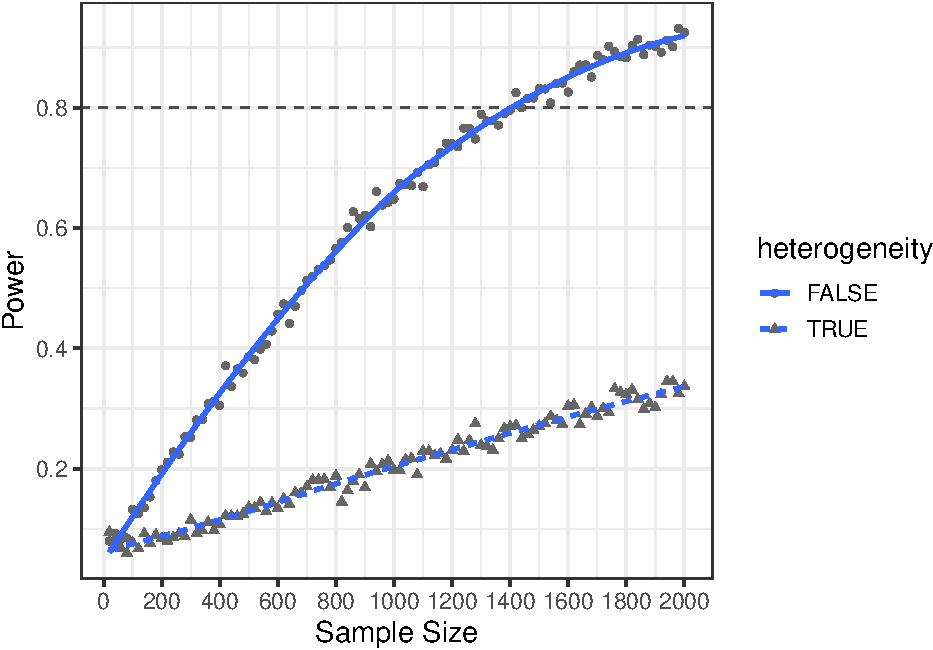
\includegraphics{power_simulation_files/figure-latex/simglm-power-curve-h-1.pdf}
\caption{\label{fig:simglm-power-curve-h}Power estimates for a single effect size (0.15) by differing sample sizes and whether there is variance heterogeneity.}
\end{figure}

\hypertarget{repeated-measures-example}{%
\section{Repeated Measures Example}\label{repeated-measures-example}}

For more complicated designs, closed form solutions are not always possible as ways to estimate statistical power or they make strong assumptions on the data that may not be reasonable given the data that are to be collected. The data simulation for the repeated measures portion adds a hierarchical data structure in which repeated measures are nested within individuals. These type of data add a correlation structure that needs to be modeled appropriately for valid inferences. Modern models to handle this dependency include the linear mixed model (LMM) (Fitzmaurice, Laird, \& Ware, 2012), sometimes known as the hierarchical linear model (HLM) (Raudenbush \& Bryk, 2002) or multilevel model (Goldstein, 2011).

This framework is an extension of the linear model considered above in the two group model. The extension includes the addition of random effects which represent subject specific deviations from the average trejectories. These random effects are what account for the dependency due to repeated measurements and nested data structure. In addition to the addition of random effects, two sample sizes need to be given, one representing the number of measurement occasions for each individual and another representing how individuals to generate. Therefore, in the balanced case (i.e.~same number of measurement occasions for each individual), the total sample size (i.e.~number of rows in the data) will be the number of measurement occasions times the number of individuals. This is a good initial check to ensure that the number of records are correct.

The code below also introduces a new argument to the fixed and randomeffect arguments, called \texttt{var\_level} which indicates at which level the variable belongs to. The default value is level 1 which would represent the repeated measures and level 2 would represent individuals. In this case, the sex variable and the random effects need to be specified at level 2 or the individual level (i.e.~these values should be constant for an individual not vary within an individual). This is done for these variables by setting \texttt{var\_level\ =\ 2}. Similarly, the sample sizes are specified for level 1 and level 2 separately in the \texttt{sample\_size} argument with \texttt{level1\ =\ 10} and \texttt{level2\ =\ 500} respectively.

\begin{Shaded}
\begin{Highlighting}[]
\NormalTok{sim_arguments <-}\StringTok{ }\KeywordTok{list}\NormalTok{(}
  \DataTypeTok{formula =}\NormalTok{ y }\OperatorTok{~}\StringTok{ }\DecValTok{1} \OperatorTok{+}\StringTok{ }\NormalTok{time }\OperatorTok{+}\StringTok{ }\NormalTok{sex }\OperatorTok{+}\StringTok{ }\NormalTok{time}\OperatorTok{:}\NormalTok{sex }\OperatorTok{+}\StringTok{ }\NormalTok{(}\DecValTok{1} \OperatorTok{+}\StringTok{ }\NormalTok{time }\OperatorTok{|}\StringTok{ }\NormalTok{individual),}
  \DataTypeTok{reg_weights =} \KeywordTok{c}\NormalTok{(}\DecValTok{4}\NormalTok{, }\FloatTok{0.4}\NormalTok{, }\FloatTok{0.3}\NormalTok{, }\FloatTok{0.20}\NormalTok{),}
  \DataTypeTok{error =} \KeywordTok{list}\NormalTok{(}\DataTypeTok{variance =} \DecValTok{1}\NormalTok{),}
  \DataTypeTok{fixed =} \KeywordTok{list}\NormalTok{(}\DataTypeTok{time =} \KeywordTok{list}\NormalTok{(}\DataTypeTok{var_type =} \StringTok{'time'}\NormalTok{),}
               \DataTypeTok{sex =} \KeywordTok{list}\NormalTok{(}\DataTypeTok{var_type =} \StringTok{'factor'}\NormalTok{, }\DataTypeTok{levels =} \KeywordTok{c}\NormalTok{(}\StringTok{'male'}\NormalTok{, }\StringTok{'female'}\NormalTok{),}
                          \DataTypeTok{var_level =} \DecValTok{2}\NormalTok{)),}
  \DataTypeTok{randomeffect =} \KeywordTok{list}\NormalTok{(}\DataTypeTok{int_individual =} \KeywordTok{list}\NormalTok{(}\DataTypeTok{variance =} \DecValTok{1}\NormalTok{, }\DataTypeTok{var_level =} \DecValTok{2}\NormalTok{),}
                      \DataTypeTok{time_individual =} \KeywordTok{list}\NormalTok{(}\DataTypeTok{variance =} \FloatTok{0.5}\NormalTok{, }\DataTypeTok{var_level =} \DecValTok{2}\NormalTok{)),}
  \DataTypeTok{sample_size =} \KeywordTok{list}\NormalTok{(}\DataTypeTok{level1 =} \DecValTok{10}\NormalTok{, }\DataTypeTok{level2 =} \DecValTok{500}\NormalTok{)}
\NormalTok{)}

\NormalTok{longitudinal_data <-}\StringTok{ }\NormalTok{sim_arguments }\OperatorTok
\StringTok{  }\KeywordTok{simulate_fixed}\NormalTok{(}\DataTypeTok{data =} \OtherTok{NULL}\NormalTok{, .) }\OperatorTok
\StringTok{  }\KeywordTok{simulate_randomeffect}\NormalTok{(sim_arguments) }\OperatorTok
\StringTok{  }\KeywordTok{simulate_error}\NormalTok{(sim_arguments) }\OperatorTok
\StringTok{  }\KeywordTok{generate_response}\NormalTok{(sim_arguments)}
\end{Highlighting}
\end{Shaded}

The data structure for this is not shown directly as it would look very similar to that shown in Table \ref{tab:simulate-data-out}.

\hypertarget{power-for-repeated-measures}{%
\subsection{Power for Repeated Measures}\label{power-for-repeated-measures}}

The structure for power for repeated measures is very similar to that found with when doing power for the two-sample t-test. The addition of number of replications, model fitting instructions, and whether to extract model coefficients are specified with the \texttt{replications}, \texttt{model\_fit}, and \texttt{extract\_coefficients} simulation arguments respectively.

\begin{Shaded}
\begin{Highlighting}[]
\NormalTok{sim_arguments <-}\StringTok{ }\KeywordTok{list}\NormalTok{(}
  \DataTypeTok{formula =}\NormalTok{ y }\OperatorTok{~}\StringTok{ }\DecValTok{1} \OperatorTok{+}\StringTok{ }\NormalTok{time }\OperatorTok{+}\StringTok{ }\NormalTok{sex }\OperatorTok{+}\StringTok{ }\NormalTok{time}\OperatorTok{:}\NormalTok{sex }\OperatorTok{+}\StringTok{ }\NormalTok{(}\DecValTok{1} \OperatorTok{+}\StringTok{ }\NormalTok{time }\OperatorTok{|}\StringTok{ }\NormalTok{individual),}
  \DataTypeTok{reg_weights =} \KeywordTok{c}\NormalTok{(}\DecValTok{4}\NormalTok{, }\FloatTok{0.4}\NormalTok{, }\FloatTok{0.3}\NormalTok{, }\FloatTok{0.20}\NormalTok{),}
  \DataTypeTok{error =} \KeywordTok{list}\NormalTok{(}\DataTypeTok{variance =} \DecValTok{1}\NormalTok{),}
  \DataTypeTok{fixed =} \KeywordTok{list}\NormalTok{(}\DataTypeTok{time =} \KeywordTok{list}\NormalTok{(}\DataTypeTok{var_type =} \StringTok{'time'}\NormalTok{),}
               \DataTypeTok{sex =} \KeywordTok{list}\NormalTok{(}\DataTypeTok{var_type =} \StringTok{'factor'}\NormalTok{, }\DataTypeTok{levels =} \KeywordTok{c}\NormalTok{(}\StringTok{'male'}\NormalTok{, }\StringTok{'female'}\NormalTok{),}
                          \DataTypeTok{var_level =} \DecValTok{2}\NormalTok{)),}
  \DataTypeTok{randomeffect =} \KeywordTok{list}\NormalTok{(}\DataTypeTok{int_individual =} \KeywordTok{list}\NormalTok{(}\DataTypeTok{variance =} \DecValTok{1}\NormalTok{, }\DataTypeTok{var_level =} \DecValTok{2}\NormalTok{),}
                      \DataTypeTok{time_individual =} \KeywordTok{list}\NormalTok{(}\DataTypeTok{variance =} \FloatTok{0.5}\NormalTok{, }\DataTypeTok{var_level =} \DecValTok{2}\NormalTok{)),}
  \DataTypeTok{sample_size =} \KeywordTok{list}\NormalTok{(}\DataTypeTok{level1 =} \DecValTok{10}\NormalTok{, }\DataTypeTok{level2 =} \DecValTok{500}\NormalTok{),}
  \DataTypeTok{replications =} \DecValTok{1000}\NormalTok{,}
  \DataTypeTok{model_fit =} \KeywordTok{list}\NormalTok{(}\DataTypeTok{formula =}\NormalTok{ y }\OperatorTok{~}\StringTok{ }\DecValTok{1} \OperatorTok{+}\StringTok{ }\NormalTok{time }\OperatorTok{+}\StringTok{ }\NormalTok{sex }\OperatorTok{+}\StringTok{ }\NormalTok{time}\OperatorTok{:}\NormalTok{sex }\OperatorTok{+}\StringTok{ }
\StringTok{                     }\NormalTok{(}\DecValTok{1} \OperatorTok{+}\StringTok{ }\NormalTok{time }\OperatorTok{|}\StringTok{ }\NormalTok{individual), }
                   \DataTypeTok{model_function =} \StringTok{'lmer'}\NormalTok{),}
  \DataTypeTok{extract_coefficients =} \OtherTok{TRUE}
\NormalTok{)}

\NormalTok{long_models <-}\StringTok{ }\KeywordTok{replicate_simulation}\NormalTok{(sim_arguments)}
\end{Highlighting}
\end{Shaded}

The \texttt{compute\_statistics} function is again used to summarize the power estimates by the terms in the model. Power and precision summary statistics are returned directly and summarized in Table \ref{tab:long-power}. Power estimates reveal that power is above 0.8 for all variables in the model.

\begin{Shaded}
\begin{Highlighting}[]
\NormalTok{long_models }\OperatorTok
\StringTok{  }\KeywordTok{compute_statistics}\NormalTok{(sim_arguments, }\DataTypeTok{power =} \OtherTok{TRUE}\NormalTok{,}
                     \DataTypeTok{type_1_error =} \OtherTok{FALSE}\NormalTok{, }\DataTypeTok{precision =} \OtherTok{TRUE}\NormalTok{)}
\end{Highlighting}
\end{Shaded}

\begin{table}[t]

\caption{\label{tab:long-power}Statistical power and precision output obtained from the repeated measures example.}
\centering
\begin{tabular}{lrrrrrrr}
\toprule
Term & Avg Est & Power & Avg TS & Est SD & Avg SE & Precision & Repl\\
\midrule
(Intercept) & 4.0 & 1.00 & 54.60 & 0.07 & 0.07 & 1.02 & 1000\\
sex & 0.3 & 0.82 & 2.89 & 0.11 & 0.10 & 1.04 & 1000\\
time & 0.4 & 1.00 & 8.94 & 0.04 & 0.05 & 0.96 & 1000\\
time:sex & 0.2 & 0.87 & 3.11 & 0.06 & 0.06 & 0.96 & 1000\\
\bottomrule
\end{tabular}
\end{table}

\hypertarget{varying-simulation-conditions}{%
\subsubsection{Varying simulation conditions}\label{varying-simulation-conditions}}

Sample size is now varied to explore the impact that different level 1 and level 2 sample sizes have on power estimates. The \texttt{vary\_arguments} simulation argument is used to control this behavior where the level 1 sample size was specified to either be 5 or 8 measurement occasions and the level 2 sample size was varied to be either 50, 150, or 250 individuals.

\begin{Shaded}
\begin{Highlighting}[]
\NormalTok{sim_arguments <-}\StringTok{ }\KeywordTok{list}\NormalTok{(}
  \DataTypeTok{formula =}\NormalTok{ y }\OperatorTok{~}\StringTok{ }\DecValTok{1} \OperatorTok{+}\StringTok{ }\NormalTok{time }\OperatorTok{+}\StringTok{ }\NormalTok{sex }\OperatorTok{+}\StringTok{ }\NormalTok{time}\OperatorTok{:}\NormalTok{sex }\OperatorTok{+}\StringTok{ }\NormalTok{(}\DecValTok{1} \OperatorTok{+}\StringTok{ }\NormalTok{time }\OperatorTok{|}\StringTok{ }\NormalTok{individual),}
  \DataTypeTok{reg_weights =} \KeywordTok{c}\NormalTok{(}\DecValTok{4}\NormalTok{, }\FloatTok{0.4}\NormalTok{, }\FloatTok{0.3}\NormalTok{, }\FloatTok{0.20}\NormalTok{),}
  \DataTypeTok{error =} \KeywordTok{list}\NormalTok{(}\DataTypeTok{variance =} \DecValTok{1}\NormalTok{),}
  \DataTypeTok{fixed =} \KeywordTok{list}\NormalTok{(}\DataTypeTok{time =} \KeywordTok{list}\NormalTok{(}\DataTypeTok{var_type =} \StringTok{'time'}\NormalTok{),}
               \DataTypeTok{sex =} \KeywordTok{list}\NormalTok{(}\DataTypeTok{var_type =} \StringTok{'factor'}\NormalTok{, }\DataTypeTok{levels =} \KeywordTok{c}\NormalTok{(}\StringTok{'male'}\NormalTok{, }\StringTok{'female'}\NormalTok{),}
                          \DataTypeTok{var_level =} \DecValTok{2}\NormalTok{)),}
  \DataTypeTok{randomeffect =} \KeywordTok{list}\NormalTok{(}\DataTypeTok{int_individual =} \KeywordTok{list}\NormalTok{(}\DataTypeTok{variance =} \DecValTok{1}\NormalTok{, }\DataTypeTok{var_level =} \DecValTok{2}\NormalTok{),}
                      \DataTypeTok{time_individual =} \KeywordTok{list}\NormalTok{(}\DataTypeTok{variance =} \FloatTok{0.5}\NormalTok{, }\DataTypeTok{var_level =} \DecValTok{2}\NormalTok{)),}
  \DataTypeTok{replications =} \DecValTok{1000}\NormalTok{,}
  \DataTypeTok{model_fit =} \KeywordTok{list}\NormalTok{(}\DataTypeTok{formula =}\NormalTok{ y }\OperatorTok{~}\StringTok{ }\DecValTok{1} \OperatorTok{+}\StringTok{ }\NormalTok{time }\OperatorTok{+}\StringTok{ }\NormalTok{sex }\OperatorTok{+}\StringTok{ }\NormalTok{time}\OperatorTok{:}\NormalTok{sex }\OperatorTok{+}\StringTok{ }
\StringTok{                     }\NormalTok{(}\DecValTok{1} \OperatorTok{+}\StringTok{ }\NormalTok{time }\OperatorTok{|}\StringTok{ }\NormalTok{individual), }
                   \DataTypeTok{model_function =} \StringTok{'lmer'}\NormalTok{),}
  \DataTypeTok{extract_coefficients =} \OtherTok{TRUE}\NormalTok{,}
  \DataTypeTok{vary_arguments =} \KeywordTok{list}\NormalTok{(}
    \DataTypeTok{sample_size =} \KeywordTok{list}\NormalTok{(}\KeywordTok{list}\NormalTok{(}\DataTypeTok{level1 =} \DecValTok{5}\NormalTok{, }\DataTypeTok{level2 =} \DecValTok{50}\NormalTok{),}
                       \KeywordTok{list}\NormalTok{(}\DataTypeTok{level1 =} \DecValTok{5}\NormalTok{, }\DataTypeTok{level2 =} \DecValTok{150}\NormalTok{),}
                       \KeywordTok{list}\NormalTok{(}\DataTypeTok{level1 =} \DecValTok{5}\NormalTok{, }\DataTypeTok{level2 =} \DecValTok{250}\NormalTok{),}
                       \KeywordTok{list}\NormalTok{(}\DataTypeTok{level1 =} \DecValTok{8}\NormalTok{, }\DataTypeTok{level2 =} \DecValTok{50}\NormalTok{),}
                       \KeywordTok{list}\NormalTok{(}\DataTypeTok{level1 =} \DecValTok{8}\NormalTok{, }\DataTypeTok{level2 =} \DecValTok{150}\NormalTok{),}
                       \KeywordTok{list}\NormalTok{(}\DataTypeTok{level1 =} \DecValTok{8}\NormalTok{, }\DataTypeTok{level2 =} \DecValTok{250}\NormalTok{))}
\NormalTok{  )}
\NormalTok{)}

\NormalTok{long_model_nomiss <-}\StringTok{ }\KeywordTok{replicate_simulation}\NormalTok{(sim_arguments) }
\end{Highlighting}
\end{Shaded}

The summary statistics from the different sample size conditions are summarized and save in the object, \texttt{long\_power\_nomiss}.

\begin{Shaded}
\begin{Highlighting}[]
\NormalTok{long_power_nomiss <-}\StringTok{ }\NormalTok{long_model_nomiss }\OperatorTok
\StringTok{  }\KeywordTok{compute_statistics}\NormalTok{(sim_arguments, }\DataTypeTok{power =} \OtherTok{TRUE}\NormalTok{,}
                     \DataTypeTok{type_1_error =} \OtherTok{FALSE}\NormalTok{, }\DataTypeTok{precision =} \OtherTok{TRUE}\NormalTok{)}
\end{Highlighting}
\end{Shaded}

In addition to just sample size, missing data can also be added to the design with the simulation argument, \texttt{missing\_data}. Dropout missing data can be common in longitudinal designs where data from individuals stops at some point in the data collection. For example, an individual may come for the first two measurement occasions, but the subsequent measurement occasions for that individual are missing. Arguments within the \texttt{missing\_data} include the new outcome variable to include in the data object that has the missing data included called \texttt{new\_outcome}, the proportion of missing data with \texttt{miss\_prop}, the cluster variable called \texttt{clust\_var}, and the type of missing data mechanism with \texttt{type}. To call dropout missing data set \texttt{type\ =\ "dropout"}. The simglm documentation contains information on additional missing data mechanisms that are currently supported. The last aspect that needs to be modified is to use the new outcome variable when specifying the \texttt{model\_fit} simulation argument. More specifically, the outcome in the model fitting step should be \texttt{y\_miss} instead of \texttt{y} to ensure that the missing data are dropped from the model fitting procedure.

\begin{Shaded}
\begin{Highlighting}[]
\NormalTok{sim_arguments <-}\StringTok{ }\KeywordTok{list}\NormalTok{(}
  \DataTypeTok{formula =}\NormalTok{ y }\OperatorTok{~}\StringTok{ }\DecValTok{1} \OperatorTok{+}\StringTok{ }\NormalTok{time }\OperatorTok{+}\StringTok{ }\NormalTok{sex }\OperatorTok{+}\StringTok{ }\NormalTok{time}\OperatorTok{:}\NormalTok{sex }\OperatorTok{+}\StringTok{ }\NormalTok{(}\DecValTok{1} \OperatorTok{+}\StringTok{ }\NormalTok{time }\OperatorTok{|}\StringTok{ }\NormalTok{individual),}
  \DataTypeTok{reg_weights =} \KeywordTok{c}\NormalTok{(}\DecValTok{4}\NormalTok{, }\FloatTok{0.4}\NormalTok{, }\FloatTok{0.3}\NormalTok{, }\FloatTok{0.20}\NormalTok{),}
  \DataTypeTok{error =} \KeywordTok{list}\NormalTok{(}\DataTypeTok{variance =} \DecValTok{1}\NormalTok{),}
  \DataTypeTok{fixed =} \KeywordTok{list}\NormalTok{(}\DataTypeTok{time =} \KeywordTok{list}\NormalTok{(}\DataTypeTok{var_type =} \StringTok{'time'}\NormalTok{),}
               \DataTypeTok{sex =} \KeywordTok{list}\NormalTok{(}\DataTypeTok{var_type =} \StringTok{'factor'}\NormalTok{, }\DataTypeTok{levels =} \KeywordTok{c}\NormalTok{(}\StringTok{'male'}\NormalTok{, }\StringTok{'female'}\NormalTok{),}
                          \DataTypeTok{var_level =} \DecValTok{2}\NormalTok{)),}
  \DataTypeTok{randomeffect =} \KeywordTok{list}\NormalTok{(}\DataTypeTok{int_individual =} \KeywordTok{list}\NormalTok{(}\DataTypeTok{variance =} \DecValTok{1}\NormalTok{, }\DataTypeTok{var_level =} \DecValTok{2}\NormalTok{),}
                      \DataTypeTok{time_individual =} \KeywordTok{list}\NormalTok{(}\DataTypeTok{variance =} \FloatTok{0.5}\NormalTok{, }\DataTypeTok{var_level =} \DecValTok{2}\NormalTok{)),}
  \DataTypeTok{replications =} \DecValTok{1000}\NormalTok{,}
  \DataTypeTok{model_fit =} \KeywordTok{list}\NormalTok{(}\DataTypeTok{formula =}\NormalTok{ y_miss }\OperatorTok{~}\StringTok{ }\DecValTok{1} \OperatorTok{+}\StringTok{ }\NormalTok{time }\OperatorTok{+}\StringTok{ }\NormalTok{sex }\OperatorTok{+}\StringTok{ }\NormalTok{time}\OperatorTok{:}\NormalTok{sex }\OperatorTok{+}\StringTok{ }
\StringTok{                     }\NormalTok{(}\DecValTok{1} \OperatorTok{+}\StringTok{ }\NormalTok{time }\OperatorTok{|}\StringTok{ }\NormalTok{individual), }
                   \DataTypeTok{model_function =} \StringTok{'lmer'}\NormalTok{),}
  \DataTypeTok{missing_data =} \KeywordTok{list}\NormalTok{(}\DataTypeTok{new_outcome =} \StringTok{'y_miss'}\NormalTok{, }\DataTypeTok{miss_prop =} \FloatTok{.20}\NormalTok{,}
                      \DataTypeTok{clust_var =} \StringTok{'individual'}\NormalTok{, }\DataTypeTok{type =} \StringTok{'dropout'}\NormalTok{),}
  \DataTypeTok{extract_coefficients =} \OtherTok{TRUE}\NormalTok{,}
  \DataTypeTok{vary_arguments =} \KeywordTok{list}\NormalTok{(}
    \DataTypeTok{sample_size =} \KeywordTok{list}\NormalTok{(}\KeywordTok{list}\NormalTok{(}\DataTypeTok{level1 =} \DecValTok{5}\NormalTok{, }\DataTypeTok{level2 =} \DecValTok{50}\NormalTok{),}
                       \KeywordTok{list}\NormalTok{(}\DataTypeTok{level1 =} \DecValTok{5}\NormalTok{, }\DataTypeTok{level2 =} \DecValTok{150}\NormalTok{),}
                       \KeywordTok{list}\NormalTok{(}\DataTypeTok{level1 =} \DecValTok{5}\NormalTok{, }\DataTypeTok{level2 =} \DecValTok{250}\NormalTok{),}
                       \KeywordTok{list}\NormalTok{(}\DataTypeTok{level1 =} \DecValTok{8}\NormalTok{, }\DataTypeTok{level2 =} \DecValTok{50}\NormalTok{),}
                       \KeywordTok{list}\NormalTok{(}\DataTypeTok{level1 =} \DecValTok{8}\NormalTok{, }\DataTypeTok{level2 =} \DecValTok{150}\NormalTok{),}
                       \KeywordTok{list}\NormalTok{(}\DataTypeTok{level1 =} \DecValTok{8}\NormalTok{, }\DataTypeTok{level2 =} \DecValTok{250}\NormalTok{))}
\NormalTok{  )}
\NormalTok{)}

\NormalTok{long_model_miss <-}\StringTok{ }\KeywordTok{replicate_simulation}\NormalTok{(sim_arguments) }
\end{Highlighting}
\end{Shaded}

Upon simulation and model fitting, the power and precision summary statistics are calculated and the power estimates are combined for the missing and complete data conditions. Some processing to make the sample size data labels easier to read for plotting is also done.

\begin{Shaded}
\begin{Highlighting}[]
\NormalTok{long_power_miss <-}\StringTok{ }\NormalTok{long_model_miss }\OperatorTok
\StringTok{  }\KeywordTok{compute_statistics}\NormalTok{(sim_arguments, }\DataTypeTok{power =} \OtherTok{TRUE}\NormalTok{,}
                     \DataTypeTok{type_1_error =} \OtherTok{FALSE}\NormalTok{, }\DataTypeTok{precision =} \OtherTok{TRUE}\NormalTok{)}

\NormalTok{long_power_nomiss_h <-}\StringTok{ }\NormalTok{long_power_nomiss }\OperatorTok
\StringTok{  }\KeywordTok{ungroup}\NormalTok{() }\OperatorTok
\StringTok{  }\KeywordTok{mutate}\NormalTok{(}\DataTypeTok{sample_size =} \KeywordTok{gsub}\NormalTok{(}\StringTok{"^list}\CharTok{\textbackslash{}\textbackslash{}}\StringTok{(|}\CharTok{\textbackslash{}\textbackslash{}}\StringTok{)$"}\NormalTok{, }\StringTok{""}\NormalTok{, }\KeywordTok{as.character}\NormalTok{(sample_size)),}
         \DataTypeTok{missing =} \OtherTok{FALSE}\NormalTok{)}

\NormalTok{long_power_miss_h <-}\StringTok{ }\NormalTok{long_power_miss }\OperatorTok
\StringTok{  }\KeywordTok{ungroup}\NormalTok{() }\OperatorTok
\StringTok{  }\KeywordTok{mutate}\NormalTok{(}\DataTypeTok{sample_size =} \KeywordTok{gsub}\NormalTok{(}\StringTok{"^list}\CharTok{\textbackslash{}\textbackslash{}}\StringTok{(|}\CharTok{\textbackslash{}\textbackslash{}}\StringTok{)$"}\NormalTok{, }\StringTok{""}\NormalTok{, }\KeywordTok{as.character}\NormalTok{(sample_size)), }
         \DataTypeTok{missing =} \OtherTok{TRUE}\NormalTok{)}

\NormalTok{long_power_combined <-}\StringTok{ }\KeywordTok{bind_rows}\NormalTok{(long_power_nomiss_h, }
\NormalTok{                                    long_power_miss_h)}
\end{Highlighting}
\end{Shaded}

Figures \ref{fig:long-power-curve-h} and \ref{fig:long-power-curve-ts} show the power estimates by various sample size conditions and whether there was missing data for the sex and time by sex interaction effects respectively. The results show that the level 2 sample size has greater impacts on power compared to changes in the level 1 sample size. In addition, the dropout missing data has greater impacts on the time by sex interaction effect compared to the sex effect. This is not surprising as the sex effect is exploring changes in the intercept based on whether the individual is male or female. In general across all of the conditions, power does not reach the often desired level of 0.80, but is closer for the time by sex interaction with the largest sample sizes.

\begin{Shaded}
\begin{Highlighting}[]
\NormalTok{long_power_sex <-}\StringTok{ }\KeywordTok{filter}\NormalTok{(long_power_combined, term }\OperatorTok{==}\StringTok{ 'sex'}\NormalTok{)}

\KeywordTok{ggplot}\NormalTok{(long_power_sex, }\KeywordTok{aes}\NormalTok{(}\DataTypeTok{x =} \KeywordTok{reorder}\NormalTok{(sample_size, }\KeywordTok{desc}\NormalTok{(power)), }\DataTypeTok{y =}\NormalTok{ power, }
                          \DataTypeTok{group =}\NormalTok{ missing)) }\OperatorTok{+}\StringTok{ }
\StringTok{  }\KeywordTok{geom_point}\NormalTok{(}\KeywordTok{aes}\NormalTok{(}\DataTypeTok{shape =}\NormalTok{ missing), }\DataTypeTok{size =} \FloatTok{1.5}\NormalTok{, }\DataTypeTok{color =} \StringTok{'gray40'}\NormalTok{) }\OperatorTok{+}\StringTok{ }
\StringTok{  }\KeywordTok{geom_line}\NormalTok{(}\KeywordTok{aes}\NormalTok{(}\DataTypeTok{linetype =}\NormalTok{ missing), }\DataTypeTok{size =} \DecValTok{1}\NormalTok{) }\OperatorTok{+}
\StringTok{  }\KeywordTok{geom_hline}\NormalTok{(}\DataTypeTok{yintercept =} \FloatTok{0.8}\NormalTok{, }\DataTypeTok{linetype =} \DecValTok{2}\NormalTok{, }\DataTypeTok{color =} \StringTok{'gray30'}\NormalTok{) }\OperatorTok{+}\StringTok{ }
\StringTok{  }\KeywordTok{xlab}\NormalTok{(}\StringTok{"Sample Size"}\NormalTok{) }\OperatorTok{+}\StringTok{ }
\StringTok{  }\KeywordTok{scale_y_continuous}\NormalTok{(}\StringTok{"Power"}\NormalTok{, }\DataTypeTok{breaks =} \KeywordTok{seq}\NormalTok{(}\DecValTok{0}\NormalTok{, }\DecValTok{1}\NormalTok{, }\FloatTok{.2}\NormalTok{), }\DataTypeTok{limits =} \KeywordTok{c}\NormalTok{(}\DecValTok{0}\NormalTok{, }\DecValTok{1}\NormalTok{)) }\OperatorTok{+}
\StringTok{  }\KeywordTok{theme_bw}\NormalTok{(}\DataTypeTok{base_size =} \DecValTok{14}\NormalTok{) }\OperatorTok{+}\StringTok{ }
\StringTok{  }\KeywordTok{coord_flip}\NormalTok{()}
\end{Highlighting}
\end{Shaded}

\begin{figure}
\centering
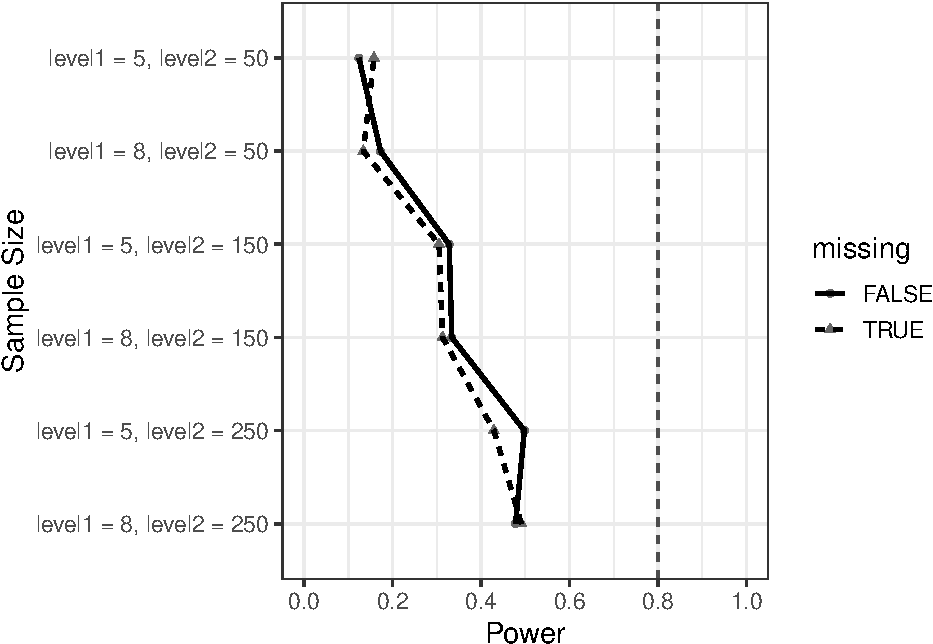
\includegraphics{power_simulation_files/figure-latex/long-power-curve-h-1.pdf}
\caption{\label{fig:long-power-curve-h}Power estimates for different sample sizes and whether missing data is included for the sex effect.}
\end{figure}

\begin{Shaded}
\begin{Highlighting}[]
\NormalTok{long_power_timesex <-}\StringTok{ }\KeywordTok{filter}\NormalTok{(long_power_combined, term }\OperatorTok{==}\StringTok{ 'time:sex'}\NormalTok{)}

\KeywordTok{ggplot}\NormalTok{(long_power_timesex, }\KeywordTok{aes}\NormalTok{(}\DataTypeTok{x =} \KeywordTok{reorder}\NormalTok{(sample_size, }\KeywordTok{desc}\NormalTok{(power)), }\DataTypeTok{y =}\NormalTok{ power, }
                          \DataTypeTok{group =}\NormalTok{ missing)) }\OperatorTok{+}\StringTok{ }
\StringTok{  }\KeywordTok{geom_point}\NormalTok{(}\KeywordTok{aes}\NormalTok{(}\DataTypeTok{shape =}\NormalTok{ missing), }\DataTypeTok{size =} \FloatTok{1.5}\NormalTok{, }\DataTypeTok{color =} \StringTok{'gray40'}\NormalTok{) }\OperatorTok{+}\StringTok{ }
\StringTok{  }\KeywordTok{geom_line}\NormalTok{(}\KeywordTok{aes}\NormalTok{(}\DataTypeTok{linetype =}\NormalTok{ missing), }\DataTypeTok{size =} \DecValTok{1}\NormalTok{) }\OperatorTok{+}
\StringTok{  }\KeywordTok{geom_hline}\NormalTok{(}\DataTypeTok{yintercept =} \FloatTok{0.8}\NormalTok{, }\DataTypeTok{linetype =} \DecValTok{2}\NormalTok{, }\DataTypeTok{color =} \StringTok{'gray30'}\NormalTok{) }\OperatorTok{+}\StringTok{ }
\StringTok{  }\CommentTok{#geom_smooth(aes(linetype = missing), size = 1, se = FALSE) +}
\StringTok{  }\CommentTok{#geom_vline(xintercept = 1488, linetype = 2, color = 'gray30') +}
\StringTok{  }\KeywordTok{xlab}\NormalTok{(}\StringTok{"Sample Size"}\NormalTok{) }\OperatorTok{+}\StringTok{ }
\StringTok{  }\KeywordTok{scale_y_continuous}\NormalTok{(}\StringTok{"Power"}\NormalTok{, }\DataTypeTok{breaks =} \KeywordTok{seq}\NormalTok{(}\DecValTok{0}\NormalTok{, }\DecValTok{1}\NormalTok{, }\FloatTok{.2}\NormalTok{), }\DataTypeTok{limits =} \KeywordTok{c}\NormalTok{(}\DecValTok{0}\NormalTok{, }\DecValTok{1}\NormalTok{)) }\OperatorTok{+}
\StringTok{  }\KeywordTok{theme_bw}\NormalTok{(}\DataTypeTok{base_size =} \DecValTok{14}\NormalTok{) }\OperatorTok{+}\StringTok{ }
\StringTok{  }\KeywordTok{coord_flip}\NormalTok{()}
\end{Highlighting}
\end{Shaded}

\begin{figure}
\centering
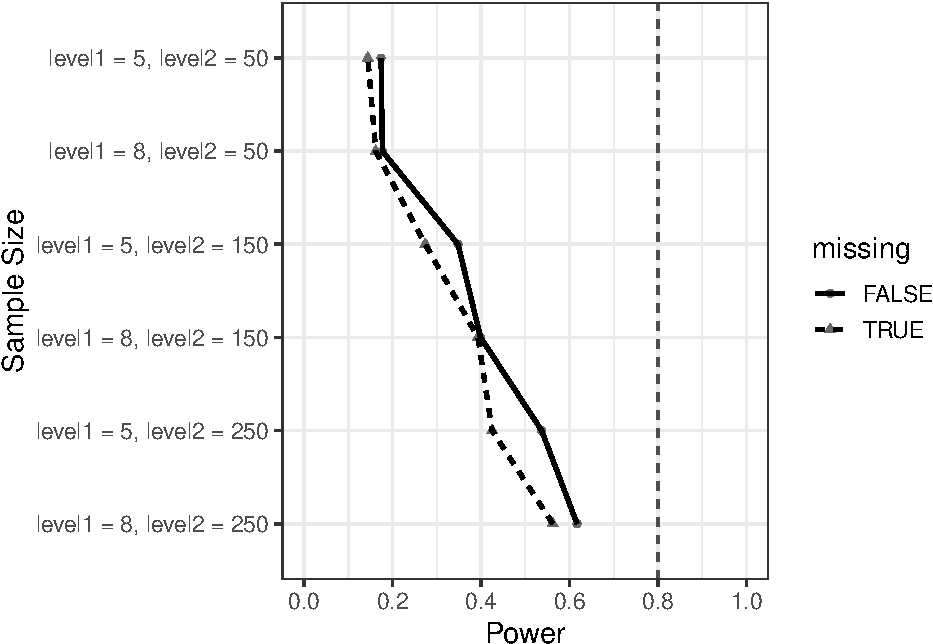
\includegraphics{power_simulation_files/figure-latex/long-power-curve-ts-1.pdf}
\caption{\label{fig:long-power-curve-ts}Power estimates for different sample sizes and whether missing data is included for the time by sex interaction.}
\end{figure}

\hypertarget{summary}{%
\section{Summary}\label{summary}}

This paper works through power examples in the traditional framework first, then explores how to generate power estimates through simulation for the two-sample t-test and repeated measures frameworks. When statistical assumptions held, the power estimates were similar between the traditional and simulation frameworks (see \ref{fig:power-figure} \ref{fig:simglm-power-curve}). This is not surprising given the assumptions that closed form power solutions make to estimate power.

The benefits of estimating power through a simulation framework occurs with the flexibility that the procedure has and the ability to mimic real world data conditions. In addition, there are models for which closed form solutions to estimate power are not as readily available, for example generalized linear models that have outcomes that are non-normally distributed and/or not continuous are more difficult to obtain closed form solutions for power.

In this tutorial, the \texttt{simglm} R package was used for power by simulation. The \texttt{simglm} package provides a framework to simulate data from a variety of generalized linear models including models that have nested or cross-classified data structures. The package also provides users ways to replicate the simulation design, vary simulation arguments, and estimate power with wrapper functions that do not require users to have to program the replications or data summarization. Users are directed to the \texttt{simglm} documentation, vignettes, and GitHub page (\url{https://github.com/lebebr01/simglm}) for additional examples and package options. The additional options include the ability to simulate models with binary or count outcomes, add additional missing data mechanisms, add additional levels of nested or cross-classifated data structures, and generate different types of variables.

\newpage

\hypertarget{references}{%
\section{References}\label{references}}

\begingroup
\setlength{\parindent}{-0.5in}
\setlength{\leftskip}{0.5in}

\hypertarget{refs}{}
\leavevmode\hypertarget{ref-pwr}{}%
Champely, S. (2018). \emph{Pwr: Basic functions for power analysis}. Retrieved from \url{https://CRAN.R-project.org/package=pwr}

\leavevmode\hypertarget{ref-powerup}{}%
Dong, N., Kelcey, B., Maynard, R., \& Spybrook, J. (2015). \emph{PowerUp! Tool for power analysis}. Retrieved from \url{https://www.causalevaluation.org/power-analysis.html}

\leavevmode\hypertarget{ref-faul2007}{}%
Faul, F., Erdfelder, E., Lang, A.-G., \& Buchner, A. (2007). G* power 3: A flexible statistical power analysis program for the social, behavioral, and biomedical sciences. \emph{Behavior Research Methods}, \emph{39}(2), 175--191.

\leavevmode\hypertarget{ref-fitzmaurice2012}{}%
Fitzmaurice, G. M., Laird, N. M., \& Ware, J. H. (2012). \emph{Applied longitudinal analysis} (Vol. 998). John Wiley \& Sons.

\leavevmode\hypertarget{ref-goldstein2011}{}%
Goldstein, H. (2011). \emph{Multilevel statistical models} (Vol. 922). John Wiley \& Sons.

\leavevmode\hypertarget{ref-hoenig2001}{}%
Hoenig, J. M., \& Heisey, D. M. (2001). The abuse of power: The pervasive fallacy of power calculations for data analysis. \emph{The American Statistician}, \emph{55}(1), 19--24.

\leavevmode\hypertarget{ref-simglm}{}%
LeBeau, B. (2019). \emph{Simglm: Simulate models based on the generalized linear model}. Retrieved from \url{https://CRAN.R-project.org/package=simglm}

\leavevmode\hypertarget{ref-optimal}{}%
Raudenbush, S., Spybrook, J., Bloom, H., Congdon, R., Hill, C., \& Martínez, A. (2011). \emph{Optimal design software for multi-level and longitudinal research}. Retrieved from \url{http://hlmsoft.net/od/}

\leavevmode\hypertarget{ref-raudenbush2002}{}%
Raudenbush, S. W., \& Bryk, A. S. (2002). \emph{Hierarchical linear models: Applications and data analysis methods} (Vol. 1). Sage.

\leavevmode\hypertarget{ref-rpro}{}%
R Core Team. (2019). \emph{R: A language and environment for statistical computing}. Vienna, Austria: R Foundation for Statistical Computing. Retrieved from \url{https://www.R-project.org/}

\leavevmode\hypertarget{ref-thomas1997}{}%
Thomas, L. (1997). Retrospective power analysis. \emph{Conservation Biology}, \emph{11}(1), 276--280.

\leavevmode\hypertarget{ref-ggplot2}{}%
Wickham, H. (2016). \emph{Ggplot2: Elegant graphics for data analysis}. Springer-Verlag New York. Retrieved from \url{http://ggplot2.org}

\leavevmode\hypertarget{ref-webpower}{}%
Zhang, Z., \& Mai, Y. (2018). \emph{WebPower: Basic and advanced statistical power analysis}. Retrieved from \url{https://CRAN.R-project.org/package=WebPower}

\endgroup


\end{document}
